\PassOptionsToPackage{quiet}{fontspec}
\documentclass[12pt,a4paper,UTF8]{article}
\usepackage{thesis} % 格式控制
\usepackage{indentfirst}
\setlength{\parindent}{2em} % 控制首行缩进
\addtolength{\parskip}{3pt} % 控制段落距离
\onehalfspacing % 1.5倍行距
\graphicspath{{./figures/}} % 指定图片所在文件夹
\pagestyle{empty}
\usepackage{enumitem}
\usepackage{multirow}
\usepackage{makecell}
\usepackage{graphicx}
\usepackage{amsmath}
\usepackage{array}
\usepackage{tabularx}
\usepackage{float}
\usepackage{xcolor}
\usepackage{listings}

\lstset{
    language=Python,
    basicstyle=\ttfamily\footnotesize,
    keywordstyle=\color{blue!60!black},
    commentstyle=\color{green!40!black},
    stringstyle=\color{orange!70!black},
    numbers=left,
    numberstyle=\tiny\color{gray},
    frame=single,
    breaklines=true,
    columns=fullflexible,
    keepspaces=true,
    showstringspaces=false,
    tabsize=4
}

\classname{算法设计与智能计算}  % 设置课程名称


\begin{document}
\maketitlepage{小组大作业}{第3小组}{施景皓~吴溪语~孙钰淳}{2026.6.6}{Min Li} % 封面页



\newpage
\pagestyle{fancy}
\fancyhf{}
\lhead{基于图最短路径与智能优化算法的玉泉校区外卖配送路径规划系统}
\chead{}
\rhead{第3小组}
\renewcommand{\headrulewidth}{0.4pt}
\cfoot{} % 无页脚，无页码

\vspace*{1em}

\begin{center}
    {\Large\bfseries 摘\quad 要}
\end{center}

\vspace{0.5em}

\setlength{\parindent}{2em}

本项目面向浙江大学玉泉校区校园跑腿配送场景，研究在校园道路拓扑、坡度变化、天气状态、货物重量和特殊地点停留惩罚共同影响下的配送路径规划问题。项目首先将玉泉校区地图抽象为有向加权图，使用节点表示校门、宿舍、食堂、教学楼、图书馆等地点以及道路交叉点，使用有向边表示道路段，并根据距离、坡度方向和坡度类型计算基础行驶时间。随后，系统在边权层面加入天气与货物重量影响，重新生成情景边代价，并通过项目内自行实现的 Dijkstra 算法预处理任意两点之间的最短行驶时间矩阵和路径矩阵。

在配送访问顺序优化层面，项目实现了最近邻贪心算法、模拟退火算法和蚁群算法三种方法，并统一使用\[total\_time = drive\_time + delay\_time\]
作为评价函数。其中，行驶时间来自当前情景下的最短路矩阵，停留时间来自完整经过路径中触发的特殊地点惩罚。为了验证启发式算法在小规模任务中的解质量，项目还实现了状态压缩动态规划精确对照算法。实验结果表明，在当前测试任务中，模拟退火算法与蚁群算法得到的路线与精确 DP 结果一致，总时间为 15.83 分钟，优于最近邻贪心算法的 19.79 分钟。最后，项目实现了 Tkinter 图形交互界面和路线可视化功能，可以根据用户输入的起点、配送点、天气、货物重量和算法类型生成路线结果、算法对比表、校园地图路线图和 GIF 动画。

\vspace{0.8em}
\noindent
\textbf{关键词：}校园配送；有向加权图；Dijkstra 算法；模拟退火；蚁群算法；动态规划；路径规划


\newpage

% —— 目录页不显示页眉页脚与页码 ——
\pagestyle{empty}
\thispagestyle{empty}
\maketoc    % 目录页

% —— 目录结束，恢复正文页眉页脚样式 ——
\pagestyle{fancy}
\fancyhf{}
\lhead{}
\chead{}
\rhead{施景皓\ 3230100613}
\renewcommand{\headrulewidth}{0.4pt}
\cfoot{\thepage}

\section{实验目的}

本实验的目标是围绕一个真实的校园配送路径规划问题，完成从问题建模、算法设计、复杂度分析到程序实现和结果展示的完整过程。与单纯求解两点之间最短路径不同，本项目需要在多个候选配送点之间确定访问顺序，同时考虑道路坡度、天气、货物重量以及经过特殊地点产生的停留惩罚。因此，该问题可以看作是在校园有向加权图上的多点配送顺序优化问题。

本实验希望达到以下目的：
\begin{enumerate}[label=(\arabic*)]
    \item 将实际校园地图抽象为程序可处理的有向加权图，建立节点、边、距离、坡度和路径之间的对应关系；
    \item 自行实现道路层最短路预处理算法，得到任意两点之间的最短行驶时间和完整路径；
    \item 在配送顺序层面实现最近邻贪心、模拟退火和蚁群算法，并比较不同算法的路线质量和运行特点；
    \item 设计天气、货物重量和特殊地点停留惩罚模型，使路线代价更接近真实校园配送场景；
    \item 使用状态压缩动态规划进行小规模精确最优解对照，验证启发式算法结果；
    \item 完成可交互的路径规划系统和路线可视化输出。
\end{enumerate}

\section{实验任务}

本实验围绕玉泉校区跑腿配送任务展开。给定一个起点、若干配送点、是否回到起点、天气类型、货物重量类型以及待使用的算法，系统需要输出一条配送访问顺序，并计算对应的行驶时间、停留时间和总时间。

输入可以表示为：
\begin{verbatim}
start: 起点
points: 配送点集合
return_to_start: 是否回到起点
weather: 天气类型
cargo: 货物重量类型
algorithm: 路线优化算法
\end{verbatim}

输出包括：
\begin{verbatim}
route: 配送访问顺序
drive_time: 情景行驶时间
delay_time: 地点停留时间
total_time: 总时间
full_path: 展开后的完整经过路径
route images: 校园地图路线图、拓扑图路线图和 GIF 动画
\end{verbatim}

为了更清楚地界定系统任务，表 \ref{tab:io_summary} 对输入与输出进行概括。可以看出，本项目的输出不仅包括一条配送访问顺序，还包括时间代价分解、算法对比结果和地图可视化结果。

\begin{table}[H]
\centering
\caption{系统输入与输出}
\label{tab:io_summary}
\small
\renewcommand{\arraystretch}{1.2}
\begin{tabularx}{\textwidth}{c|X}
\hline
类型 & 内容 \\
\hline
输入 & 起点、配送点集合、是否回到起点、天气类型、货物重量类型、待使用算法 \\
\hline
数值输出 & 配送访问顺序、行驶时间、地点停留时间、总时间、触发停留惩罚的节点 \\
\hline
对比输出 & 贪心、模拟退火、蚁群算法的路线与总耗时对比；小规模任务下的精确 DP 验证结果 \\
\hline
可视化输出 & 校园卫星地图路线图、道路拓扑图路线图、动态路线 GIF \\
\hline
\end{tabularx}
\end{table}

项目的优化目标定义为：
\[
    \min total\_time = drive\_time + delay\_time
\]
其中，\verb|drive_time| 由当前情景下的最短路矩阵查询得到，\verb|delay_time| 由完整路径经过的特殊地点触发。由于天气和货物重量对平地、上坡和下坡的影响不同，边权会随着情景改变而改变，因此系统不能只对整条路线乘统一系数，而必须基于有向边逐边重新计算情景代价。

\section{实验内容}

本实验主要包含以下内容：
\begin{enumerate}[label=(\arabic*)]
    \item 地图数据整理：根据玉泉校区地图和手工标注路线，构建包含主要地点和道路交叉点的拓扑图；
    \item 图结构构建：整理 \texttt{nodes.csv}、\texttt{edges\_raw.csv}，并将原始道路边展开为正反两个方向的有向边；
    \item 基础代价建模：根据图上距离、比例尺、电瓶车速度和坡度系数计算基础行驶时间；
    \item 情景代价建模：根据天气和货物重量逐边更新代价，并重新运行 Dijkstra；
    \item 配送路径优化：实现贪心、模拟退火和蚁群算法；
    \item 精确最优对照：使用状态压缩 DP 验证小规模任务的最优解；
    \item 系统实现：完成 UI 输入、算法运行、结果保存、地图路线图和 GIF 动画输出。
\end{enumerate}

\section{问题描述与建模}

\subsection{实际场景}

玉泉校区内不同地点之间存在坡度差异，校园配送不只受距离影响，还会受到上坡、下坡、天气、货物重量以及特殊地点停留等因素影响。例如，下雨天时下坡道路更滑，重货物在上坡时更费力；经过食堂可能因为排队产生额外停留时间，经过宿舍可能因为配送上门产生额外时间。因此，距离最短并不一定等价于配送总时间最短。

本项目将校园道路建模为有向加权图：
\[
    G=(V,E)
\]
其中，$V$ 为节点集合，包含主要地点节点和虚拟道路交叉点；$E$ 为有向边集合，每条有向边表示一段带方向的道路。由于同一段道路正反方向可能分别对应上坡和下坡，因此边权一般不对称。

\subsection{节点与边}

节点数据存放在 \texttt{data/nodes.csv} 中，当前共有 59 个节点。其中 1--19 号为主要地点节点，包括北门、菜鸟驿站、32舍、校医院、四食堂、三食堂、新桥门、8舍、永谦、田径场、教七、教一、正门、图书馆、教四、信电楼、高分子楼、曹光彪和南门；20 号及以后为道路交叉点、转弯点等虚拟节点。

引入虚拟道路节点的原因是：真实校园道路并不是主要地点之间的直线连接，若只用地点之间的直线边，会丢失道路转弯和路口结构，也无法在地图上准确绘制路线。因此项目使用虚拟节点保留道路几何结构，使最短路和可视化结果都基于同一套拓扑。

原始道路边存放在 \texttt{data/edges\_raw.csv} 中，共 81 条。每条边包含：
\begin{verbatim}
edge_id, from_id, to_id, distance, slope_type, comment
\end{verbatim}
其中，\verb|distance| 为图上标注距离，\verb|slope_type| 为坡度类型，\verb|comment| 中保存对应道路在图像上的像素线段，用于后续可视化。

每条原始边会展开成两个方向的有向边，生成 \texttt{data/directed\_edges.csv}，当前共有 162 条有向边。正反两个方向的坡度类型会根据上坡、下坡关系自动转换，因此同一段道路两个方向的代价可能不同。

当前图模型的基本规模如表 \ref{tab:graph_scale} 所示。后续 Dijkstra 最短路预处理和配送顺序优化算法均基于该图结构运行，而不是直接在地图图片上进行人工判断。

\begin{table}[H]
\centering
\caption{玉泉校区道路图模型规模}
\label{tab:graph_scale}
\small
\renewcommand{\arraystretch}{1.2}
\begin{tabularx}{0.88\textwidth}{c|c|X}
\hline
图元素 & 数量 & 含义 \\
\hline
节点 $V$ & 59 & 主要配送地点、校门、教学楼、宿舍、食堂以及道路交叉点、转弯点 \\
\hline
原始道路边 & 81 & 人工整理得到的校园道路段 \\
\hline
有向边 $E$ & 162 & 原始道路边正反方向展开后的有向边，正反方向坡度和代价可不同 \\
\hline
边权信息 & 每条边一个 & 距离、坡度类型、天气修正、货物修正后的时间代价 \\
\hline
\end{tabularx}
\end{table}

\subsection{地图构造过程}

项目的地图构造并不是直接调用地图服务或现成道路数据，而是根据玉泉校区地图逐步人工整理得到。根据实验记录，地图处理大致经历了以下几个阶段。

不直接调用地图 API 的原因是：本实验关注的是算法建模与路径优化过程，而不是调用现成导航服务。因此需要先把校园道路、地点和路口抽象为可计算的图结构，使后续所有算法都在统一的节点、边和边权数据上运行。

第一步，选取玉泉校区地图作为底图，并将地图旋转到南北方向较为规整的位置，便于后续把道路抽象成横平竖直或少量斜线的拓扑结构。第二步，在地图上手工标注北门、菜鸟驿站、32舍、校医院、食堂、教学楼、图书馆、南门等主要地点，并将手写标注整理为清晰的打印体标注。第三步，用手绘方式在地图上标出可通行道路，得到“哪些线段可以走”的道路草图。第四步，将复杂地图底图去掉，保留道路骨架，形成黑白抽象道路图。第五步，将黑白道路图进一步整理为带节点编号的正交拓扑图，并逐段标注距离。第六步，根据人工判断的上坡、下坡和平地信息，标注红色小上坡箭头、蓝色大上坡箭头和紫色平路线段，最终形成可数据化的拓扑图。

\begin{figure}[H]
    \centering
    \begin{minipage}{0.40\textwidth}
        \centering
        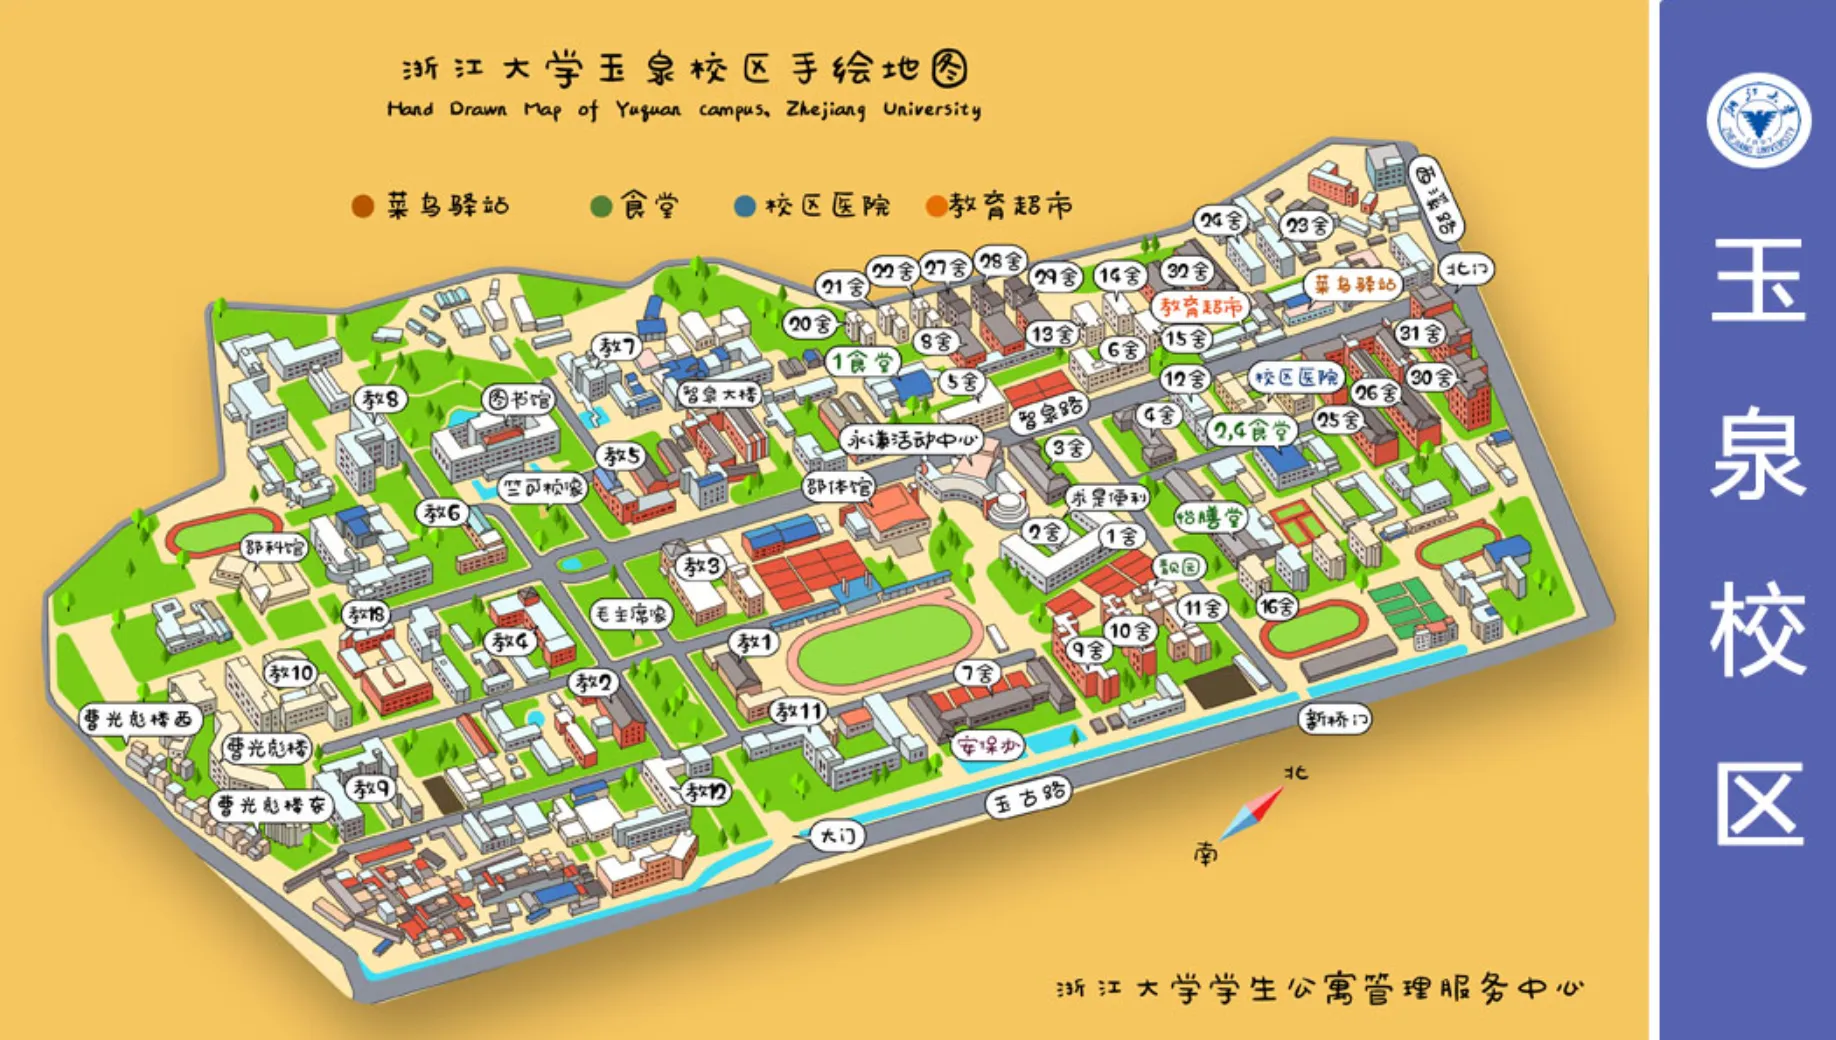
\includegraphics[width=\textwidth]{figures/report_map_first_choice.png}
        \small 最初尝试使用的玉泉校区地图
    \end{minipage}
    \hfill
    \begin{minipage}{0.40\textwidth}
        \centering
        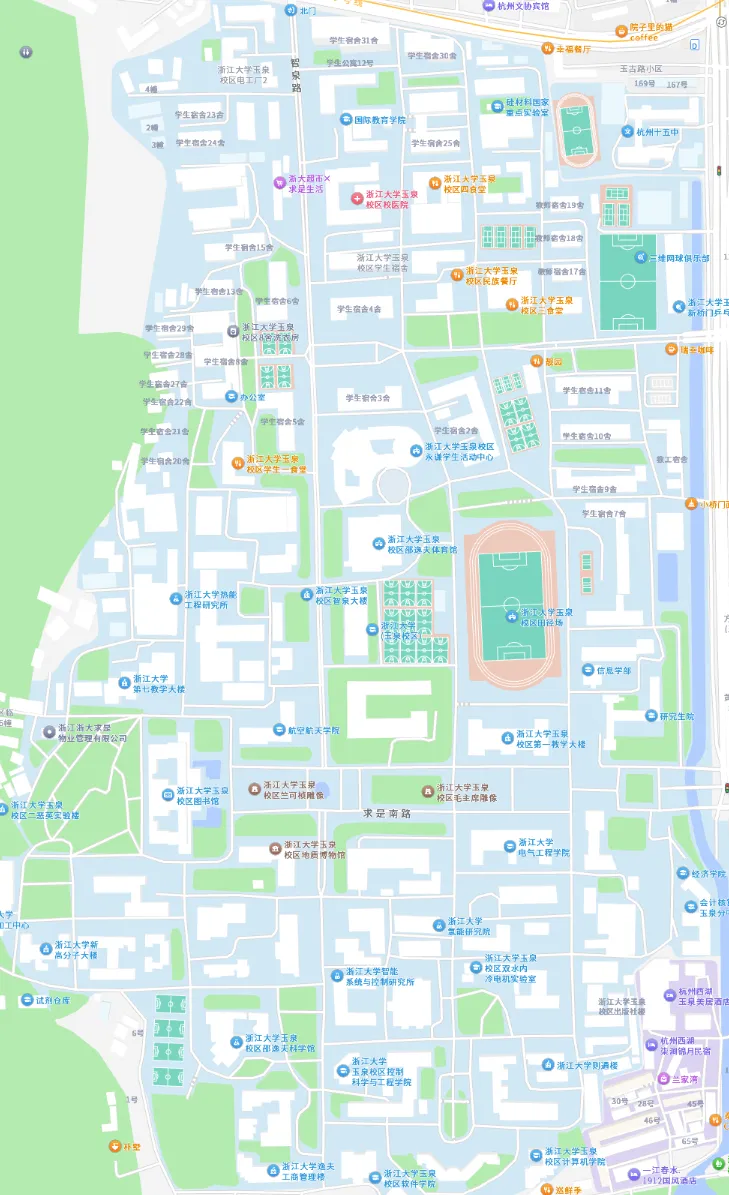
\includegraphics[width=\textwidth]{figures/report_map_satellite_rotated.png}
        \small 后续改用并旋转校正的卫星地图
    \end{minipage}

    \vspace{0.8em}

    \begin{minipage}{0.40\textwidth}
        \centering
        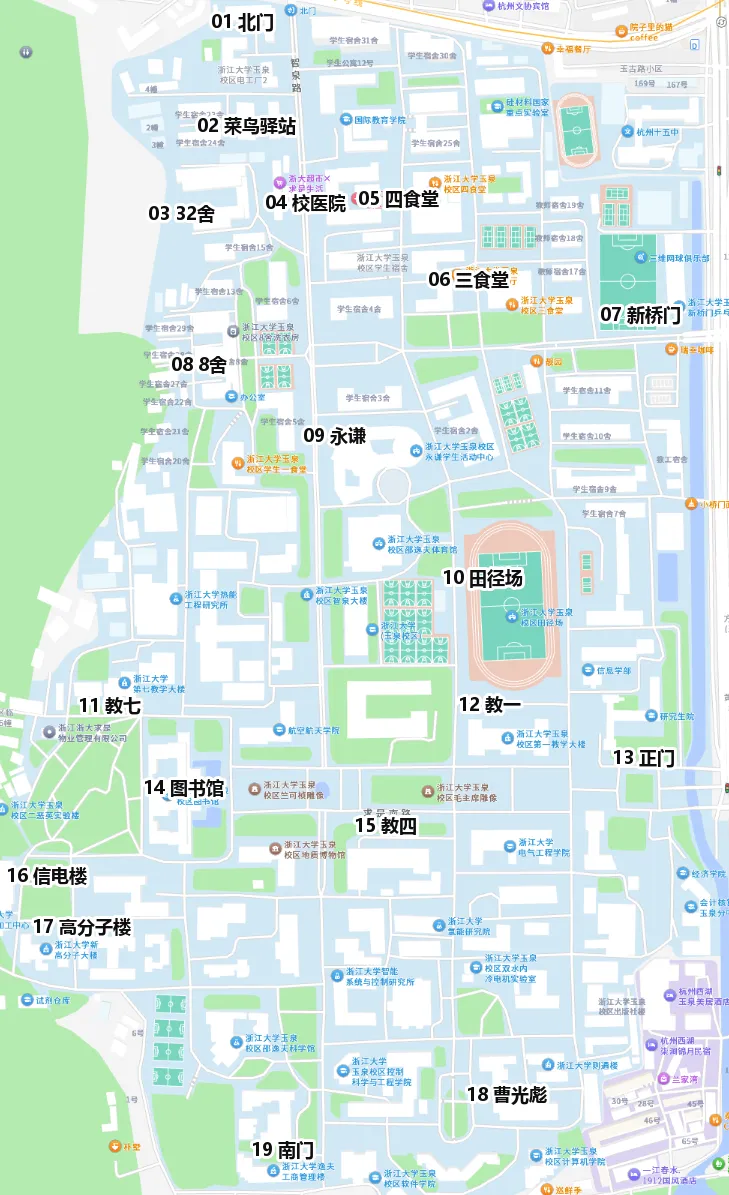
\includegraphics[width=\textwidth]{figures/report_map_labeled.png}
        \small 主要地点标注图
    \end{minipage}
    \hfill
    \begin{minipage}{0.40\textwidth}
        \centering
        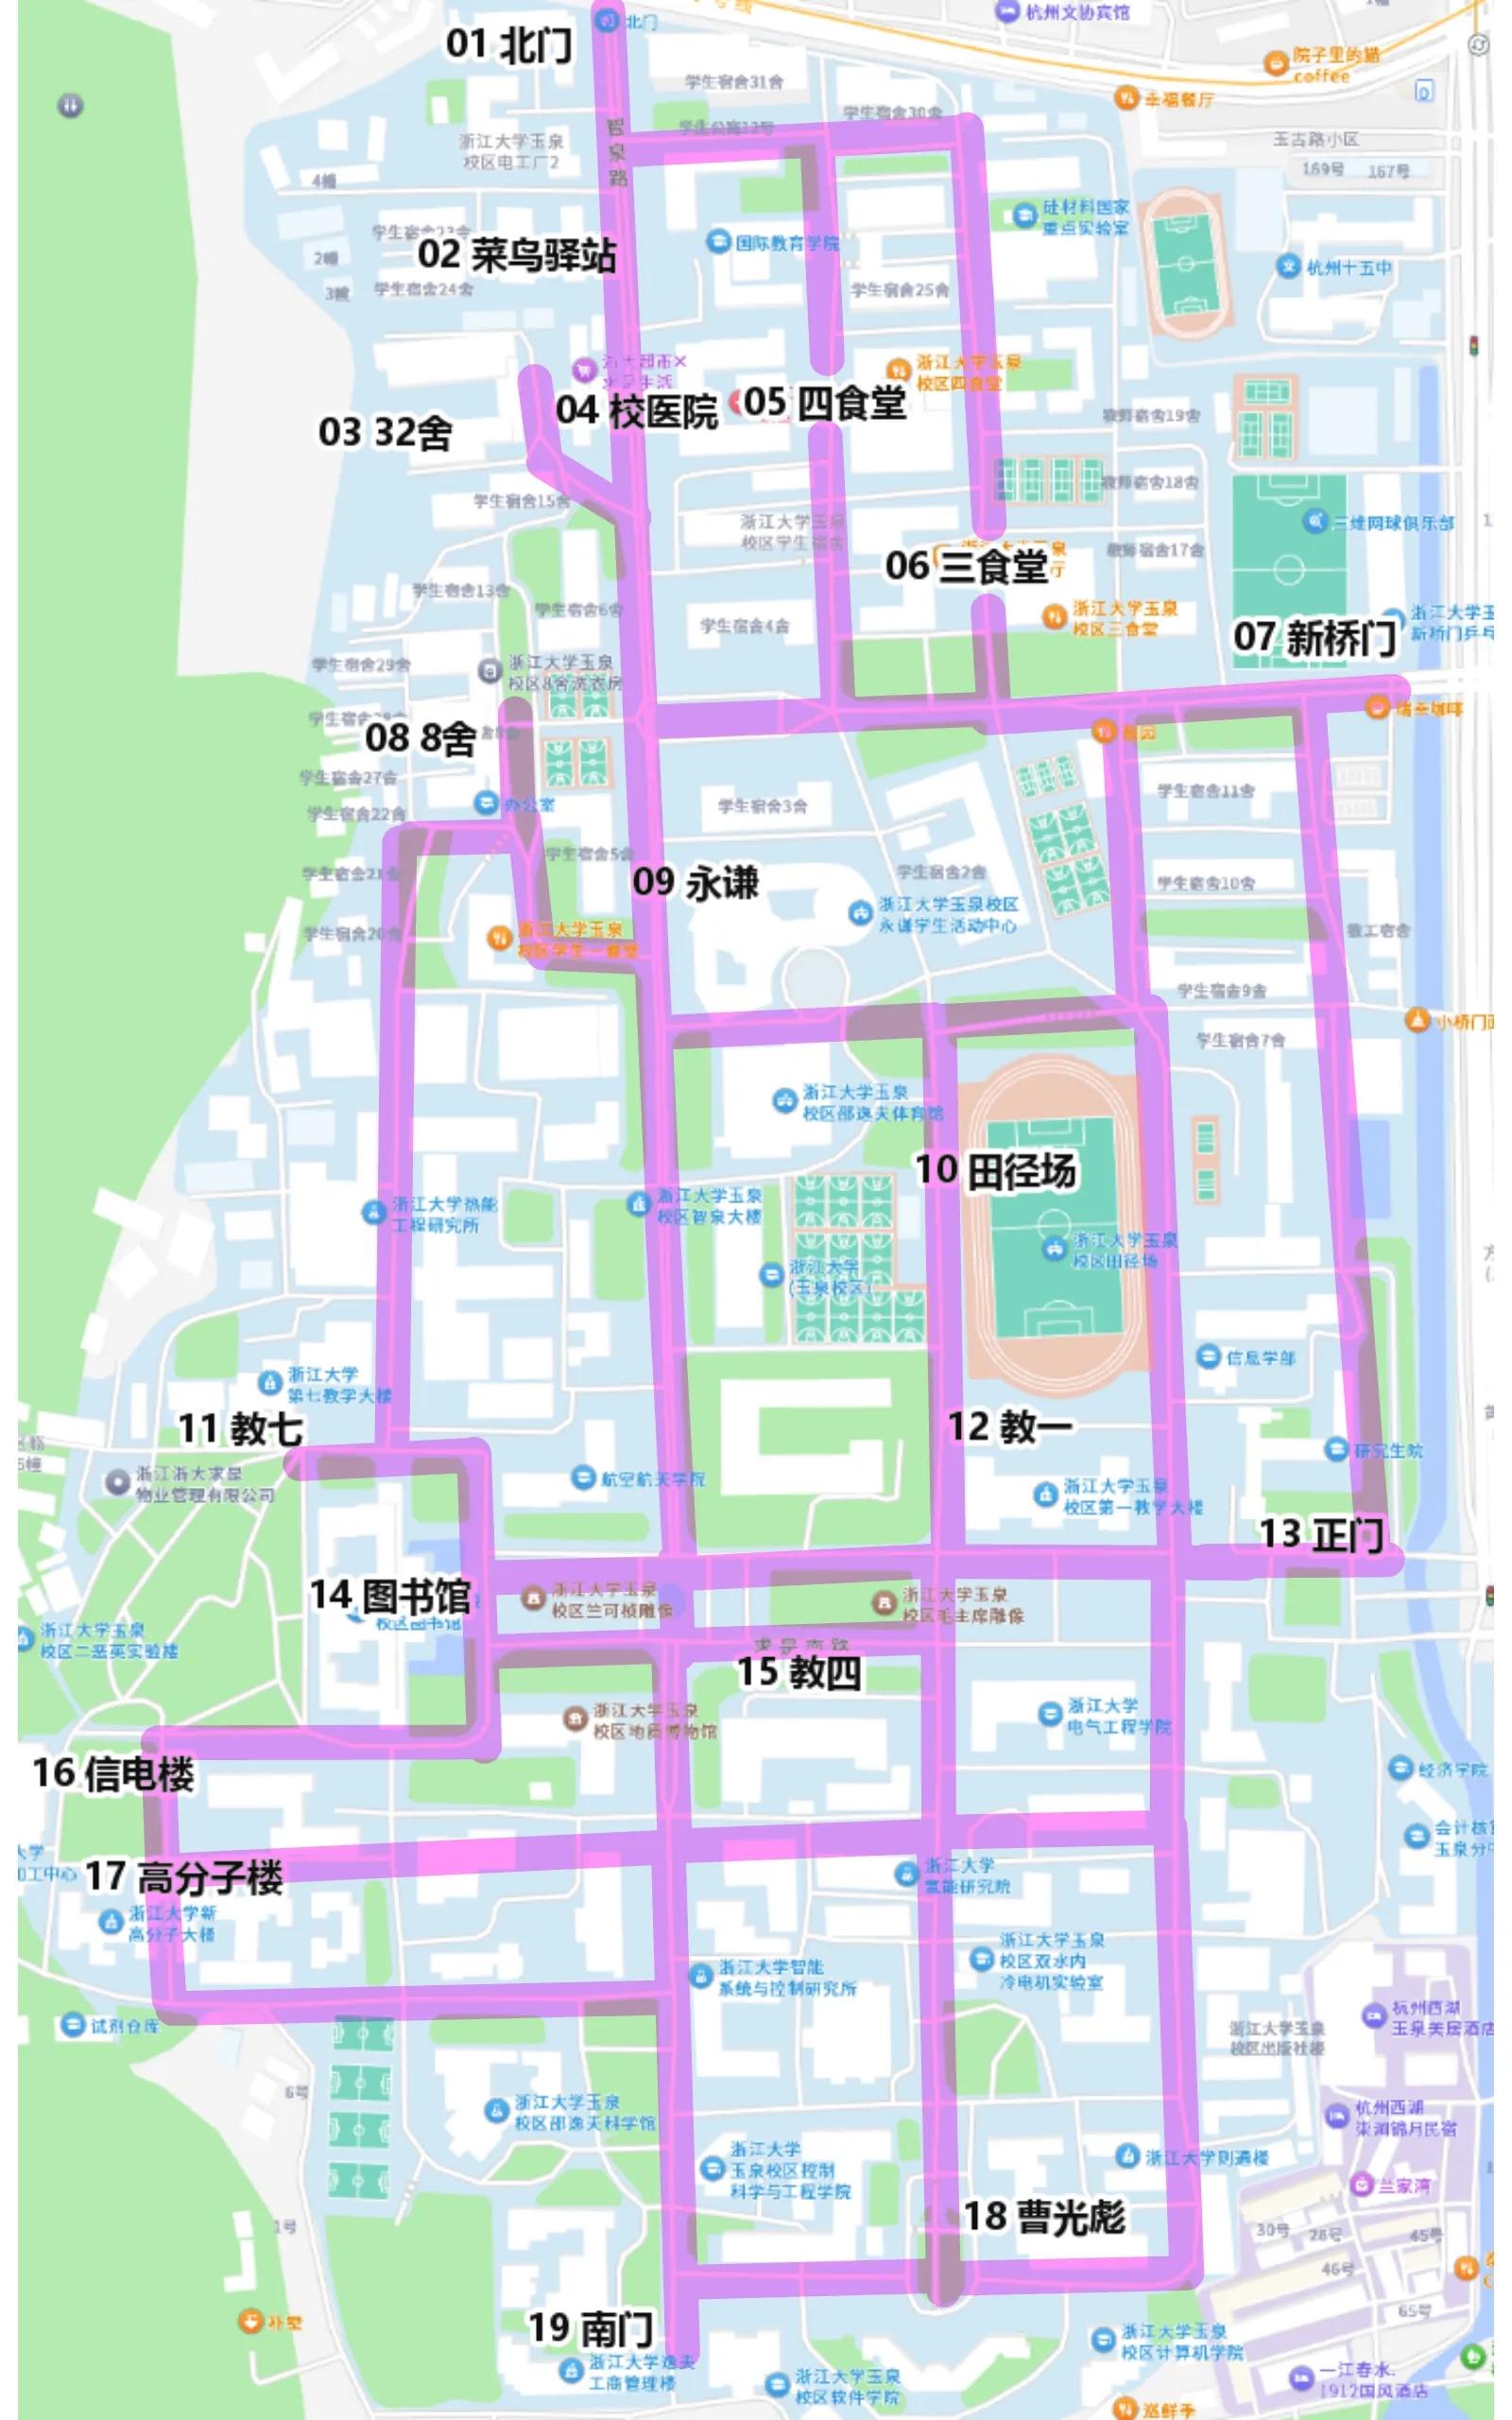
\includegraphics[width=\textwidth]{figures/report_map_hand_routes.png}
        \small 手工绘制可通行道路
    \end{minipage}
    \caption{地图底图选择、旋转校正、地点标注与道路手工标注过程}
    \label{fig:map_process}
\end{figure}

\begin{figure}[H]
    \centering
    \begin{minipage}{0.40\textwidth}
        \centering
        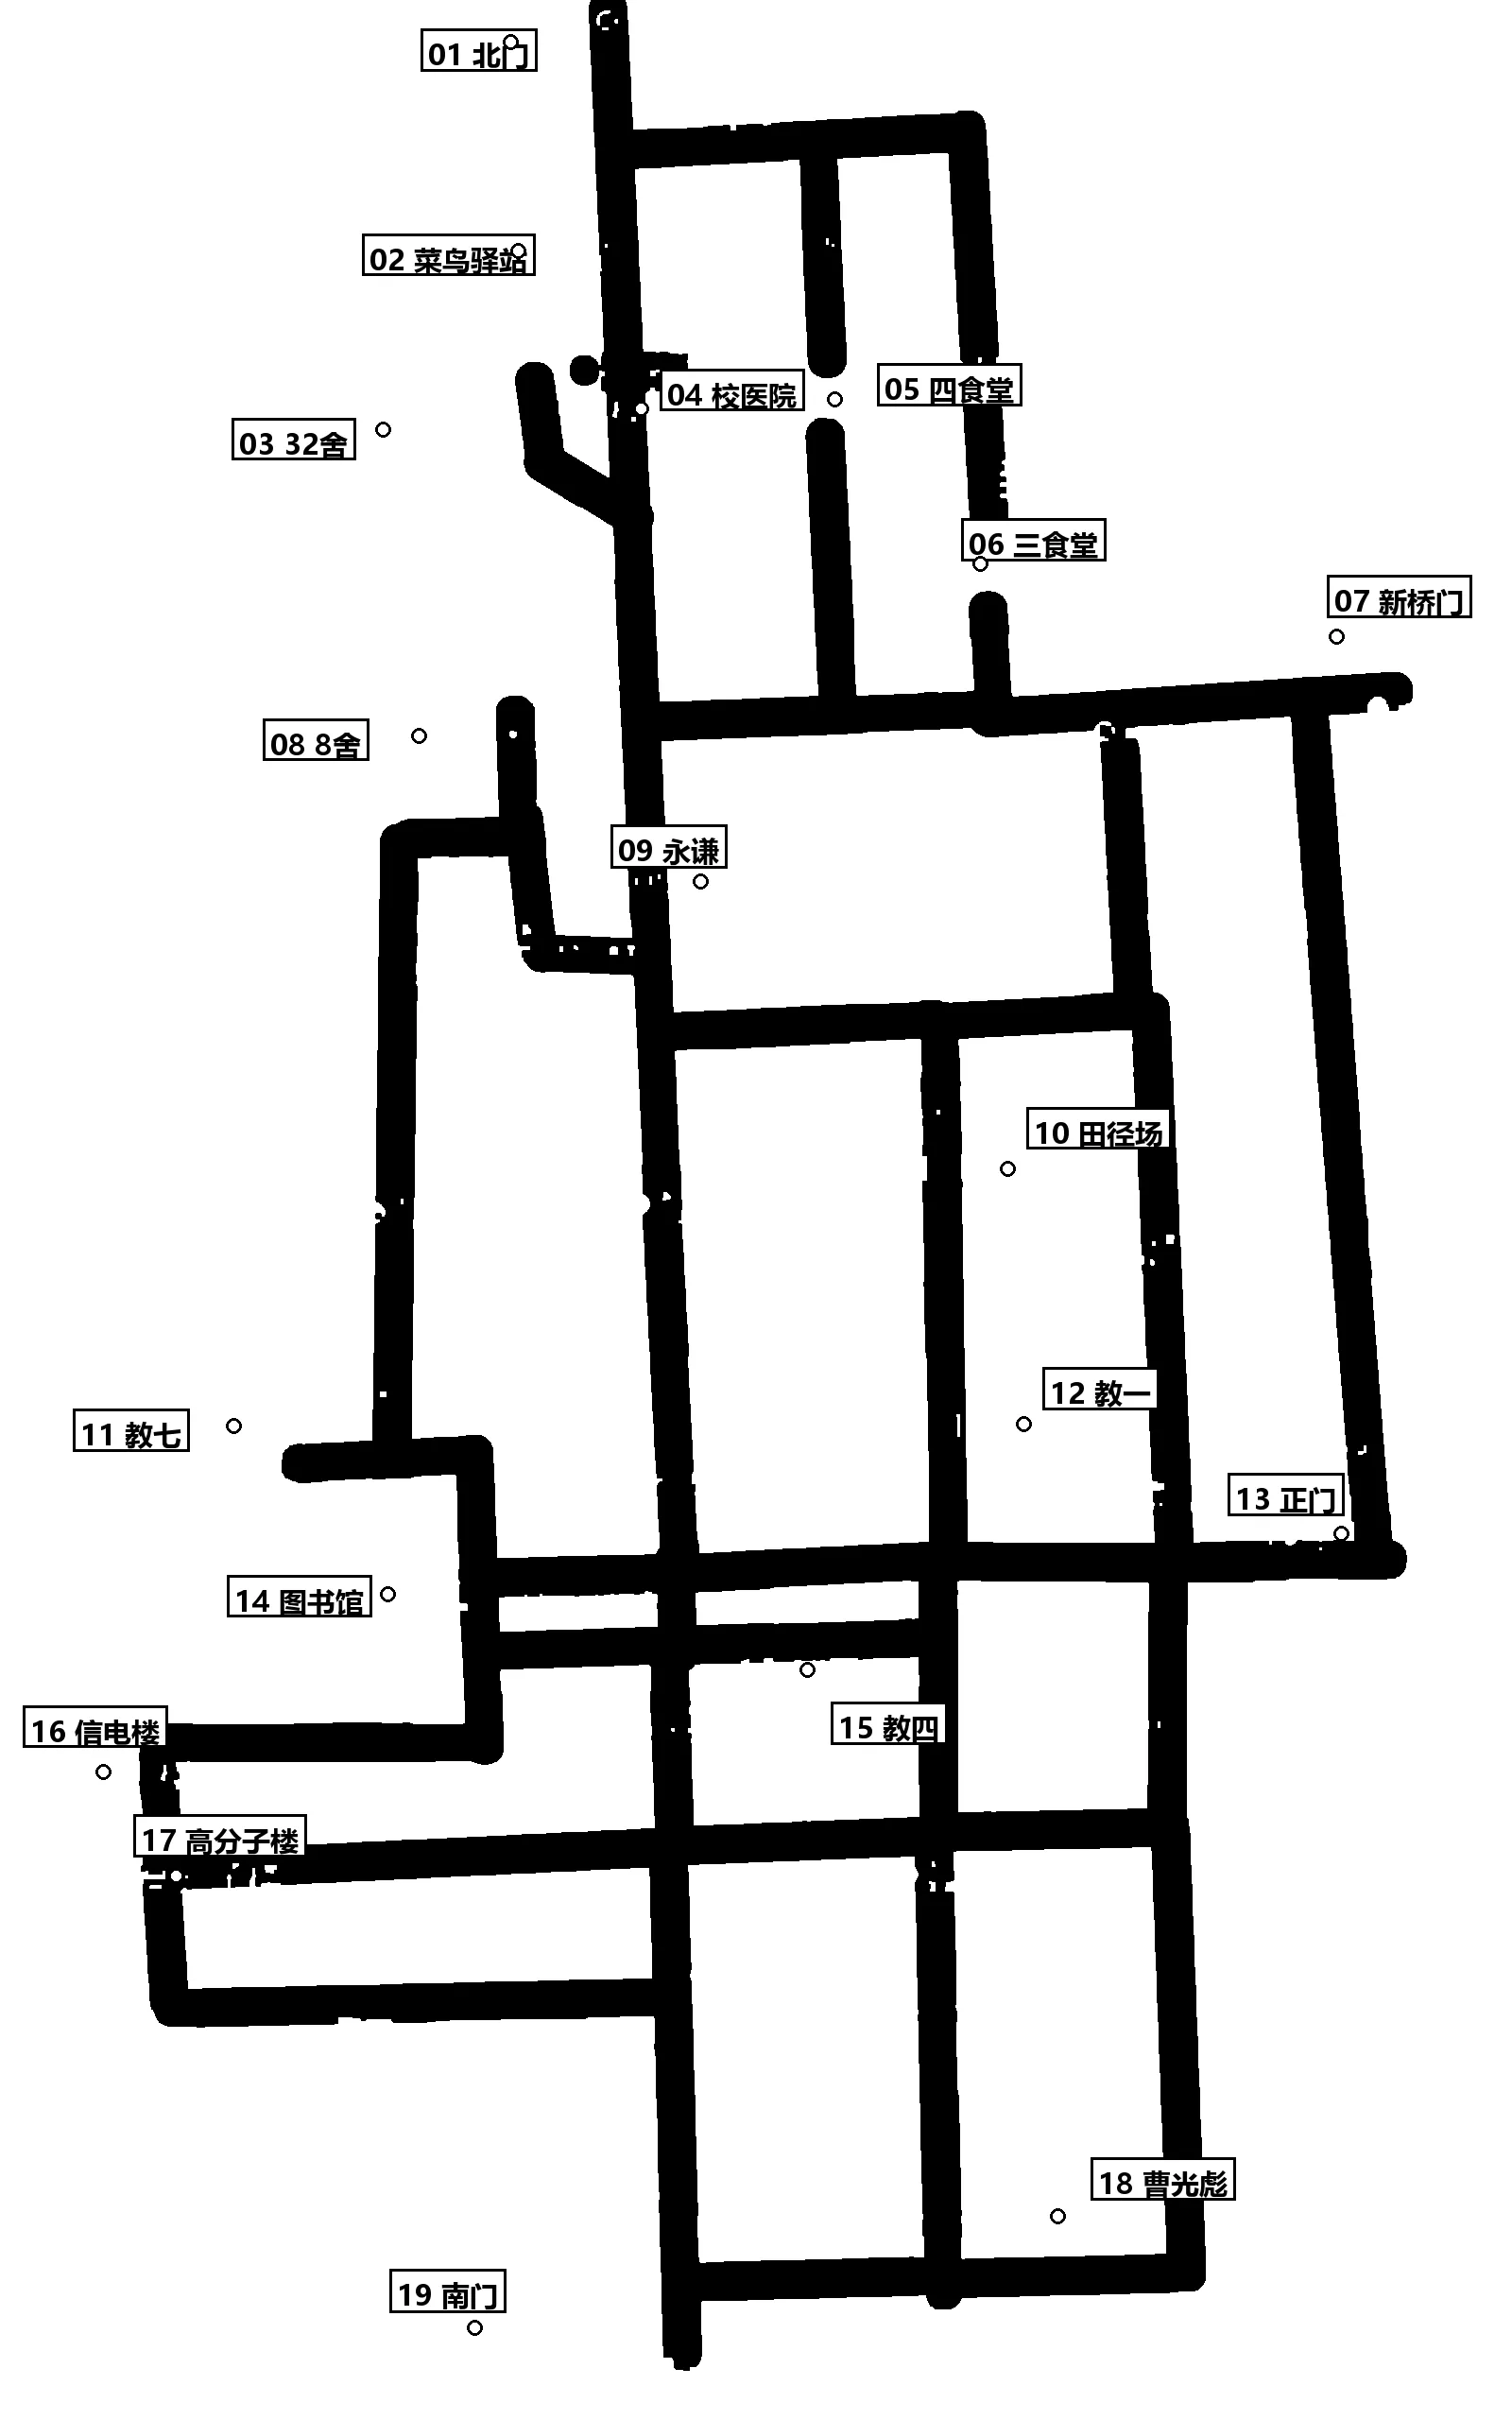
\includegraphics[width=\textwidth]{figures/report_map_blackwhite.png}
        \small 去除复杂底图后的黑白道路骨架
    \end{minipage}
    \hfill
    \begin{minipage}{0.40\textwidth}
        \centering
        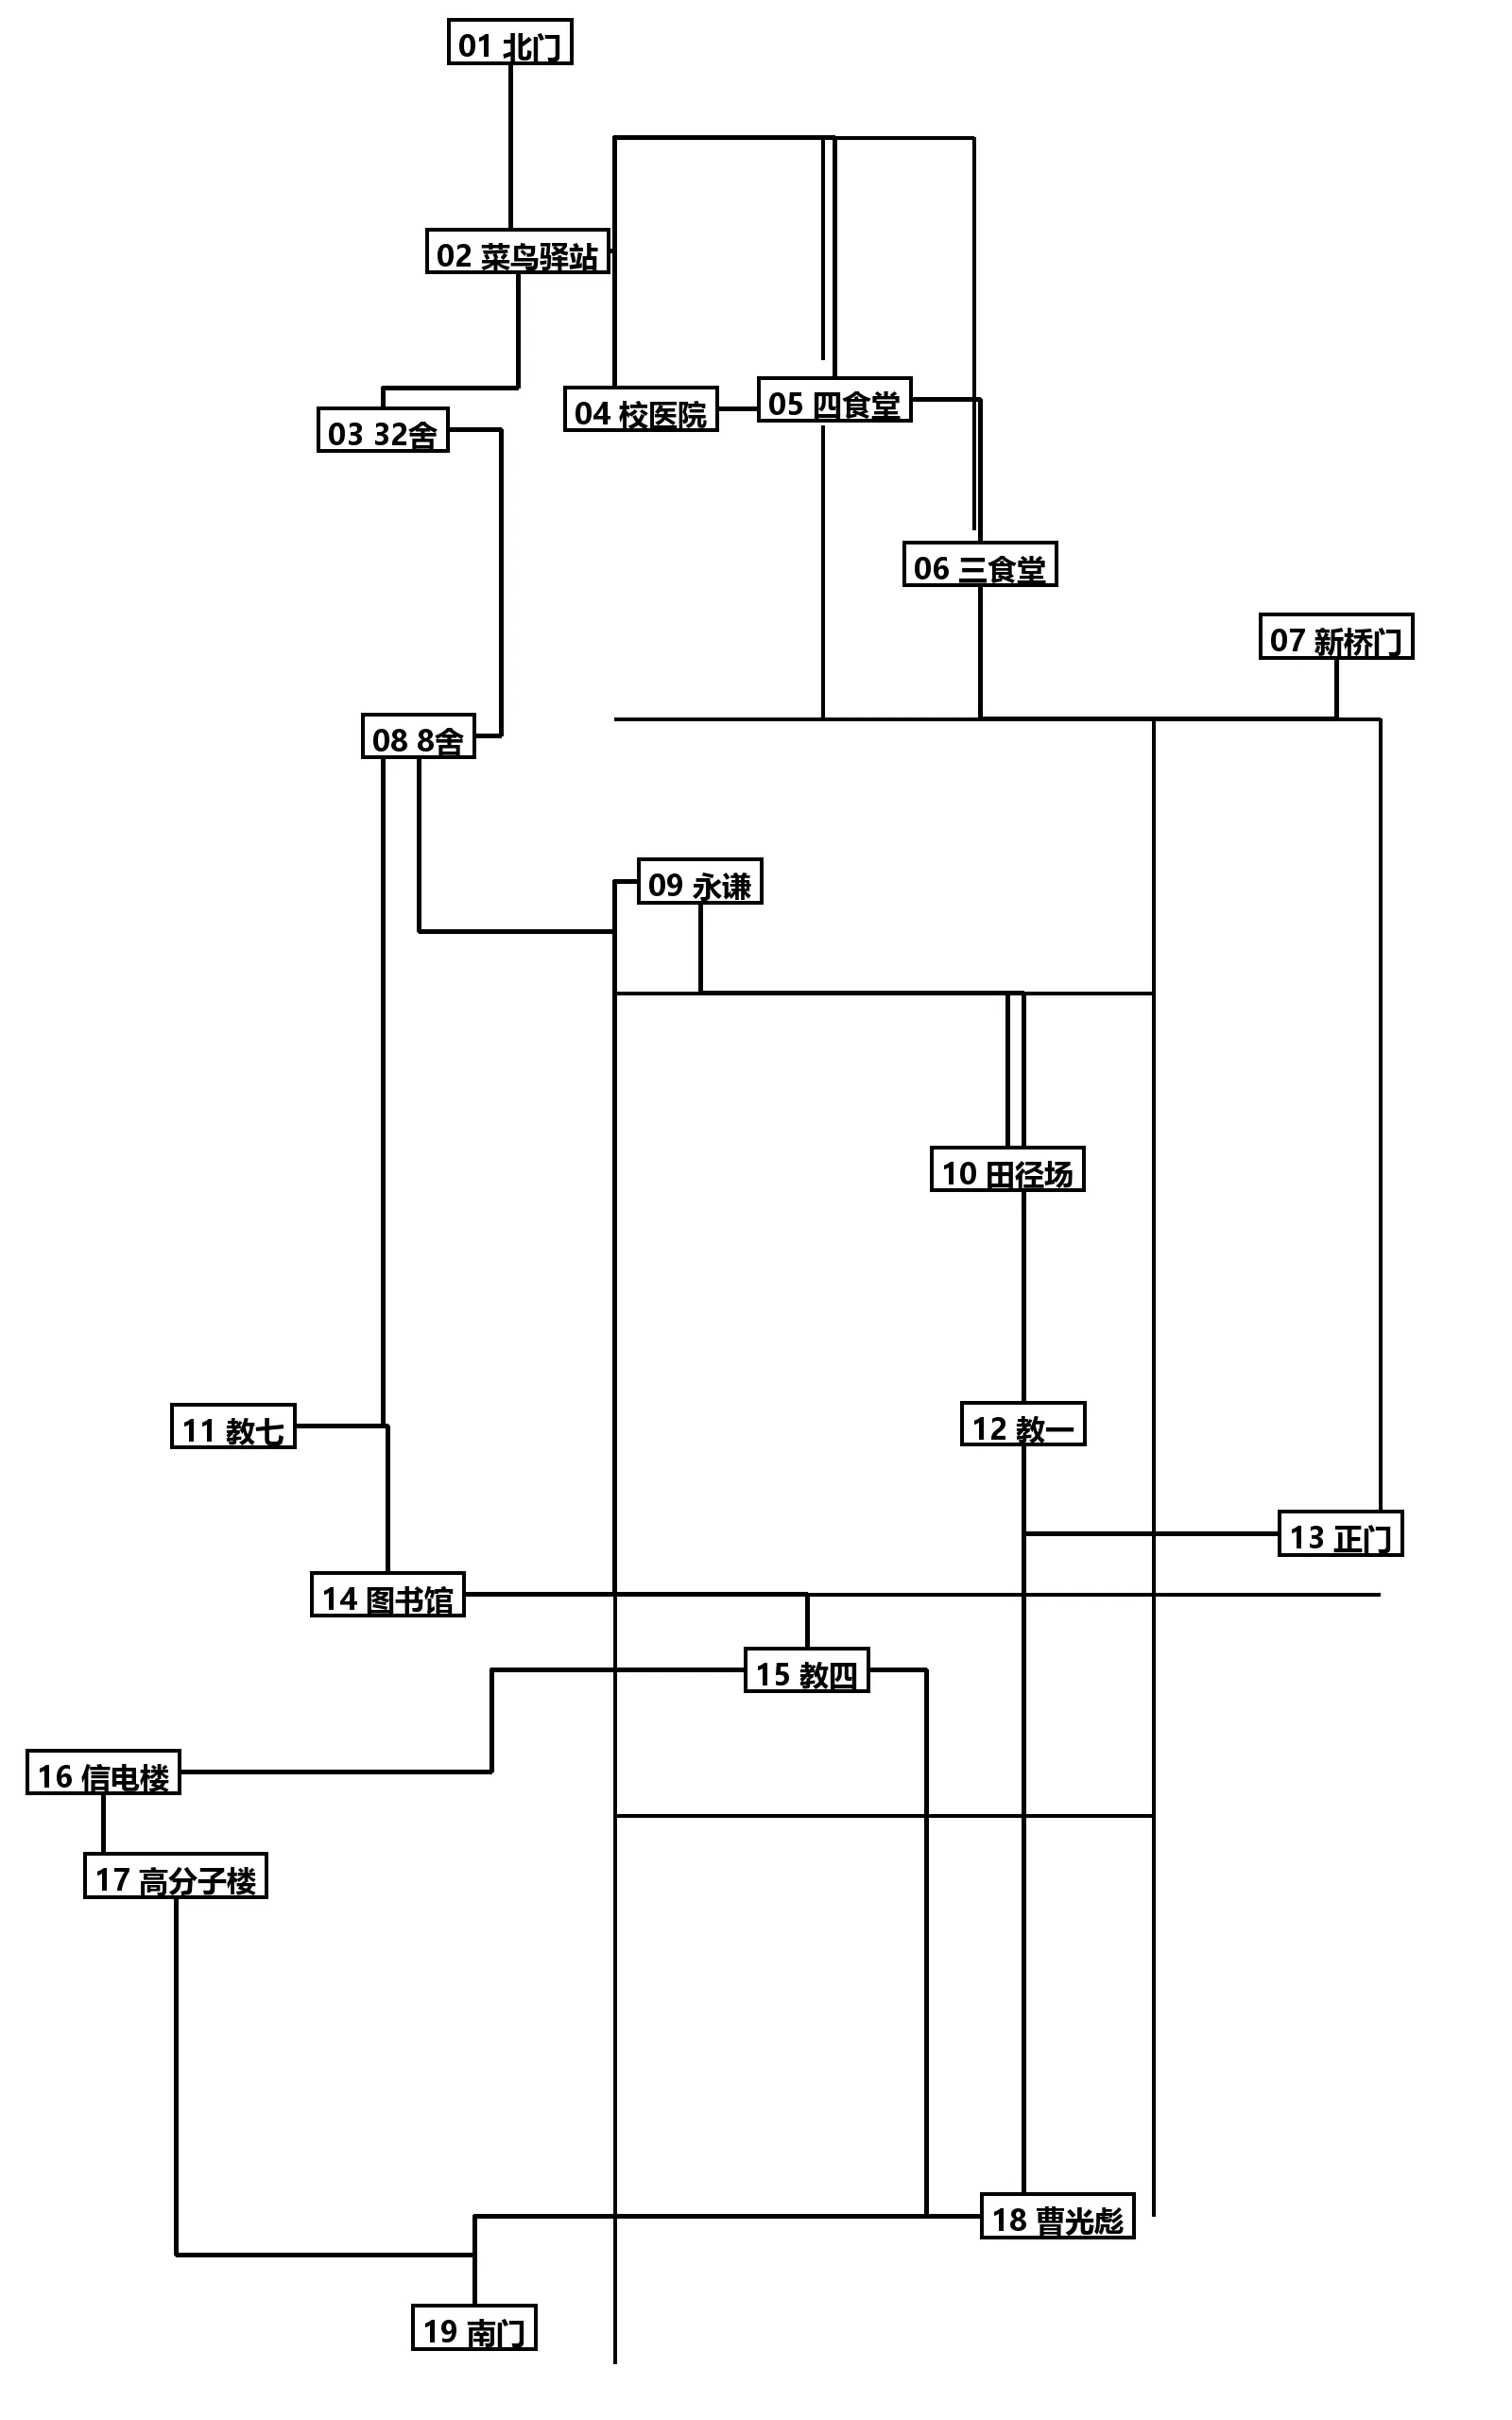
\includegraphics[width=\textwidth]{figures/report_topology_initial.png}
        \small 初步识别得到的拓扑图雏形
    \end{minipage}

    \vspace{0.8em}

    \begin{minipage}{0.40\textwidth}
        \centering
        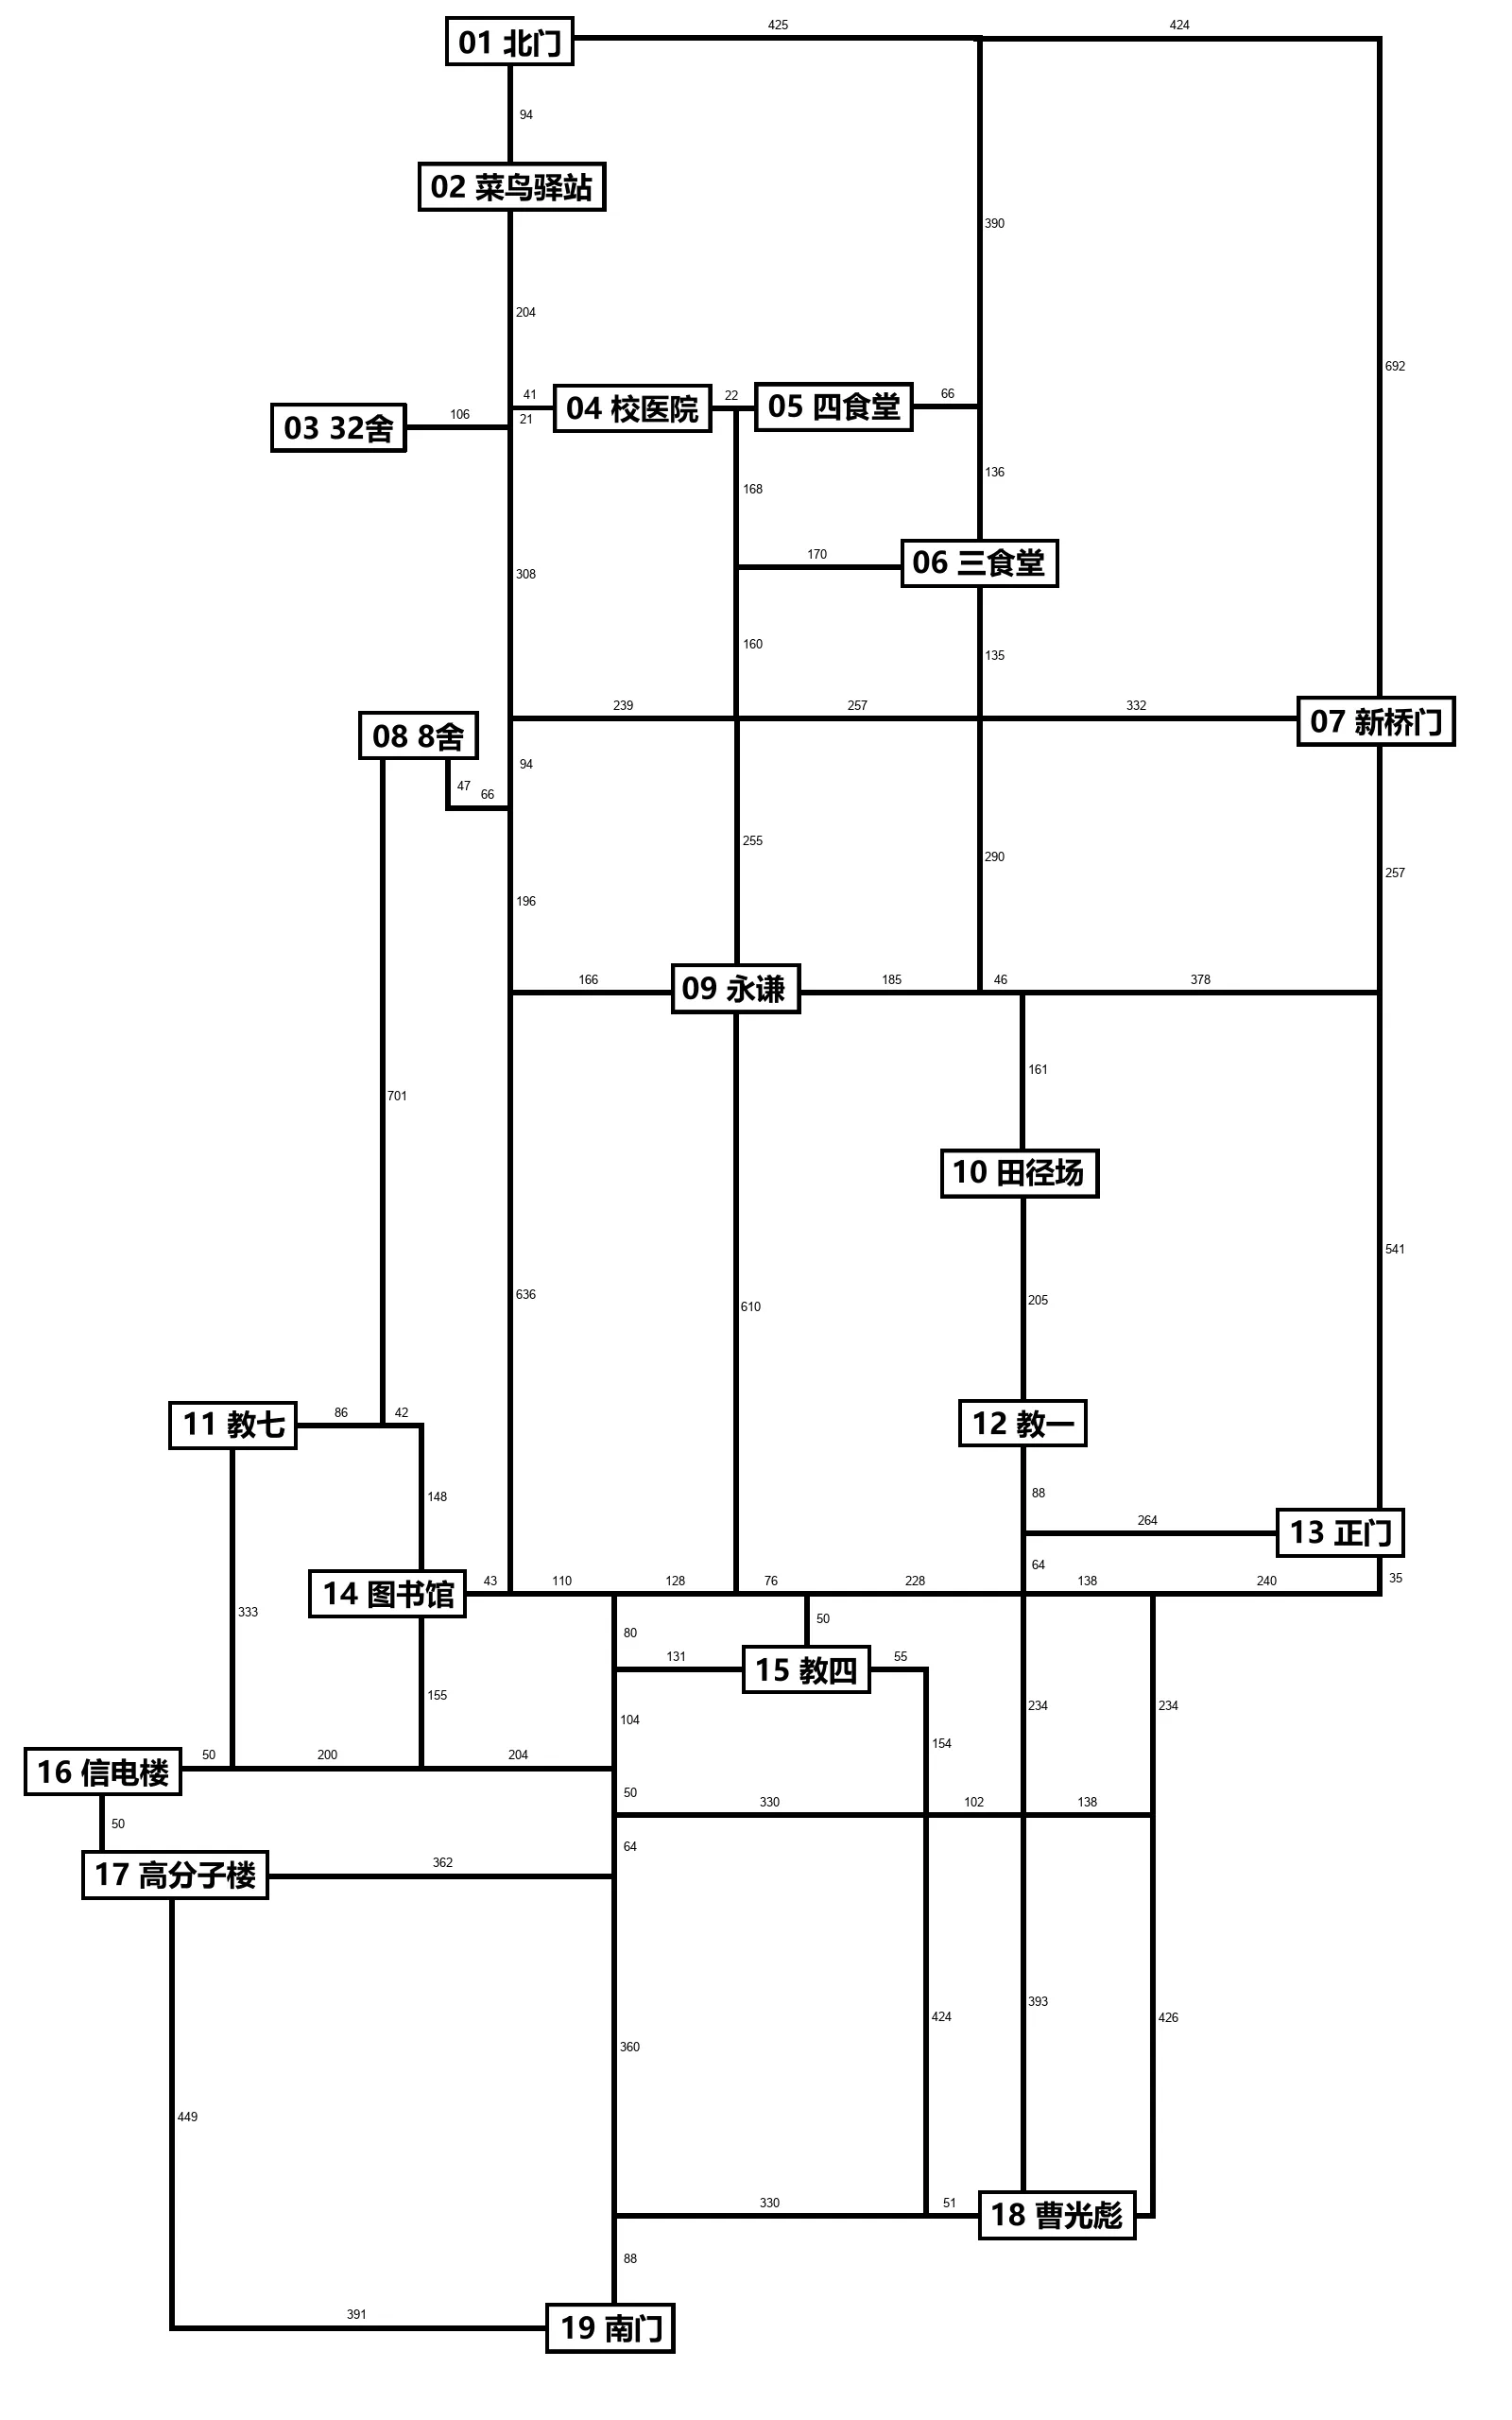
\includegraphics[width=\textwidth]{figures/report_topology_lengths.png}
        \small 路线修复与距离标注后的拓扑图
    \end{minipage}
    \hfill
    \begin{minipage}{0.40\textwidth}
        \centering
        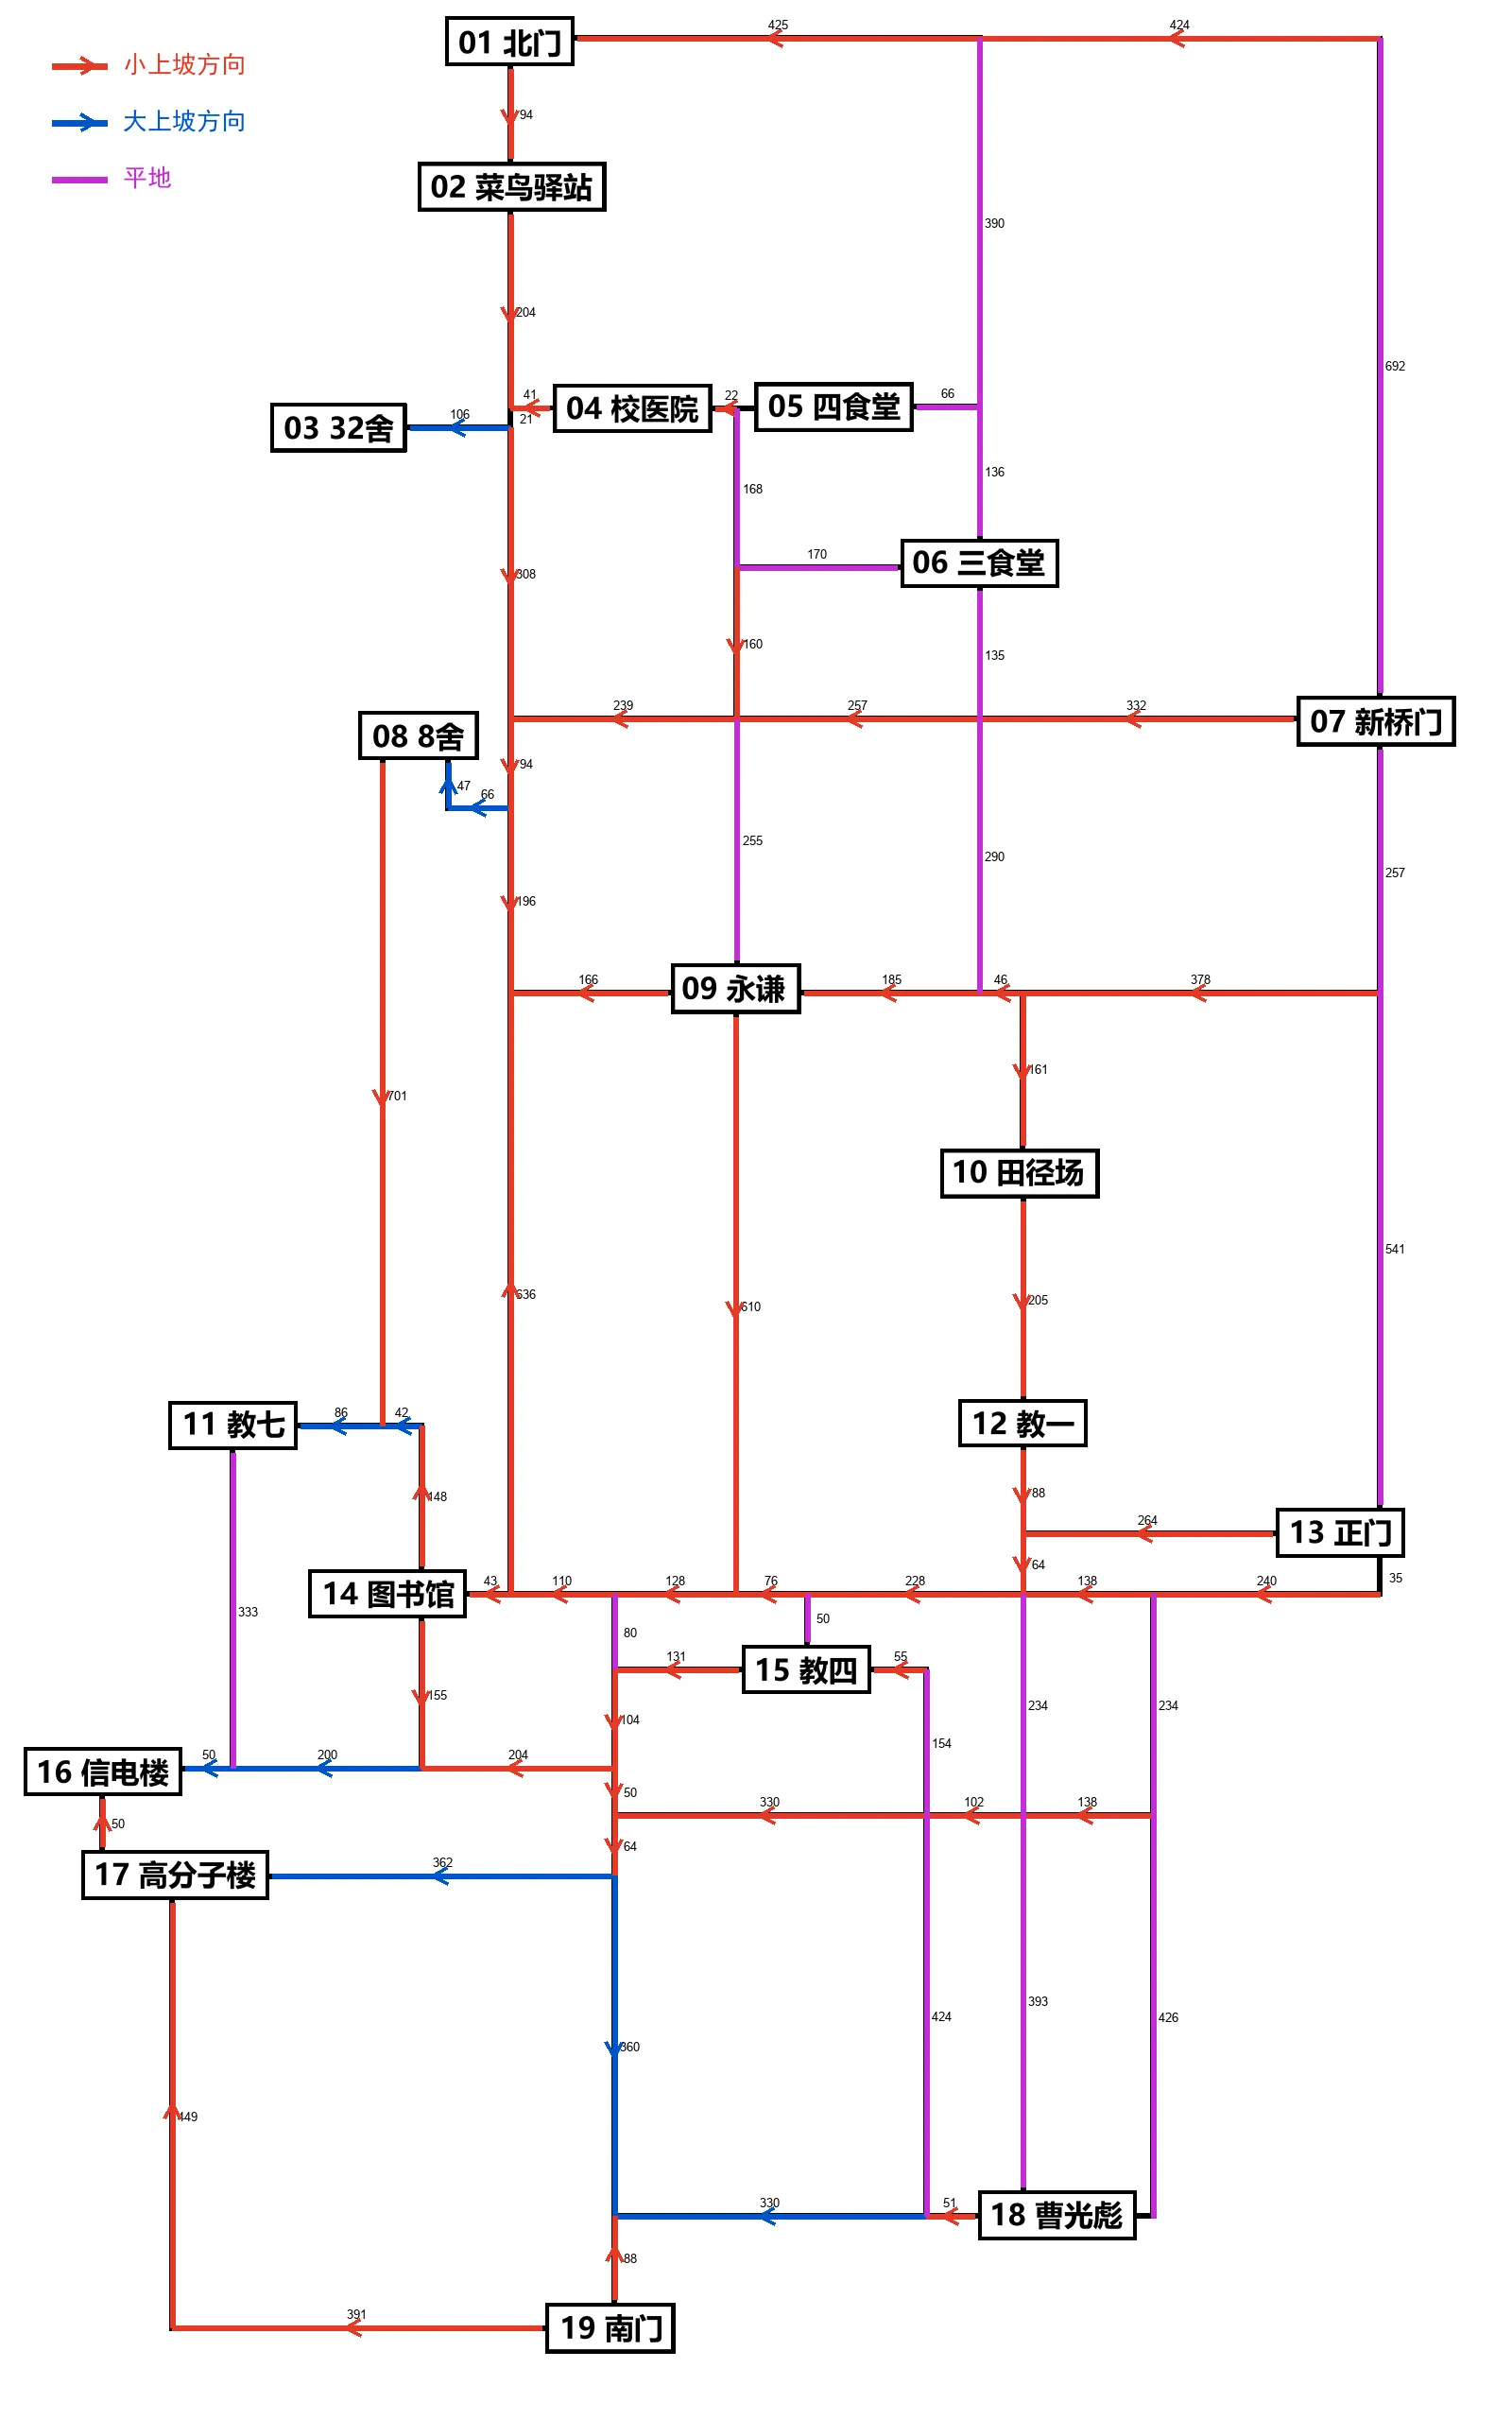
\includegraphics[width=\textwidth]{figures/report_topology_final.png}
        \small 最终采用的带距离和坡度的拓扑图
    \end{minipage}
    \caption{从黑白道路骨架到可计算拓扑图的整理过程}
    \label{fig:topology_process}
\end{figure}

在上述过程中，最关键的一步是把“图像上的路线”转换成“算法中的图结构”。例如，地图上的一条道路并不一定只连接两个地点，它可能经过多个转弯点和交叉口，因此需要补充虚拟道路节点。最终，图像中的道路线段被整理为 \texttt{edges\_raw.csv} 中的边记录，节点被整理为 \texttt{nodes.csv} 中的节点记录，距离和坡度信息则成为边权计算的基础。

\begin{figure}[H]
    \centering
    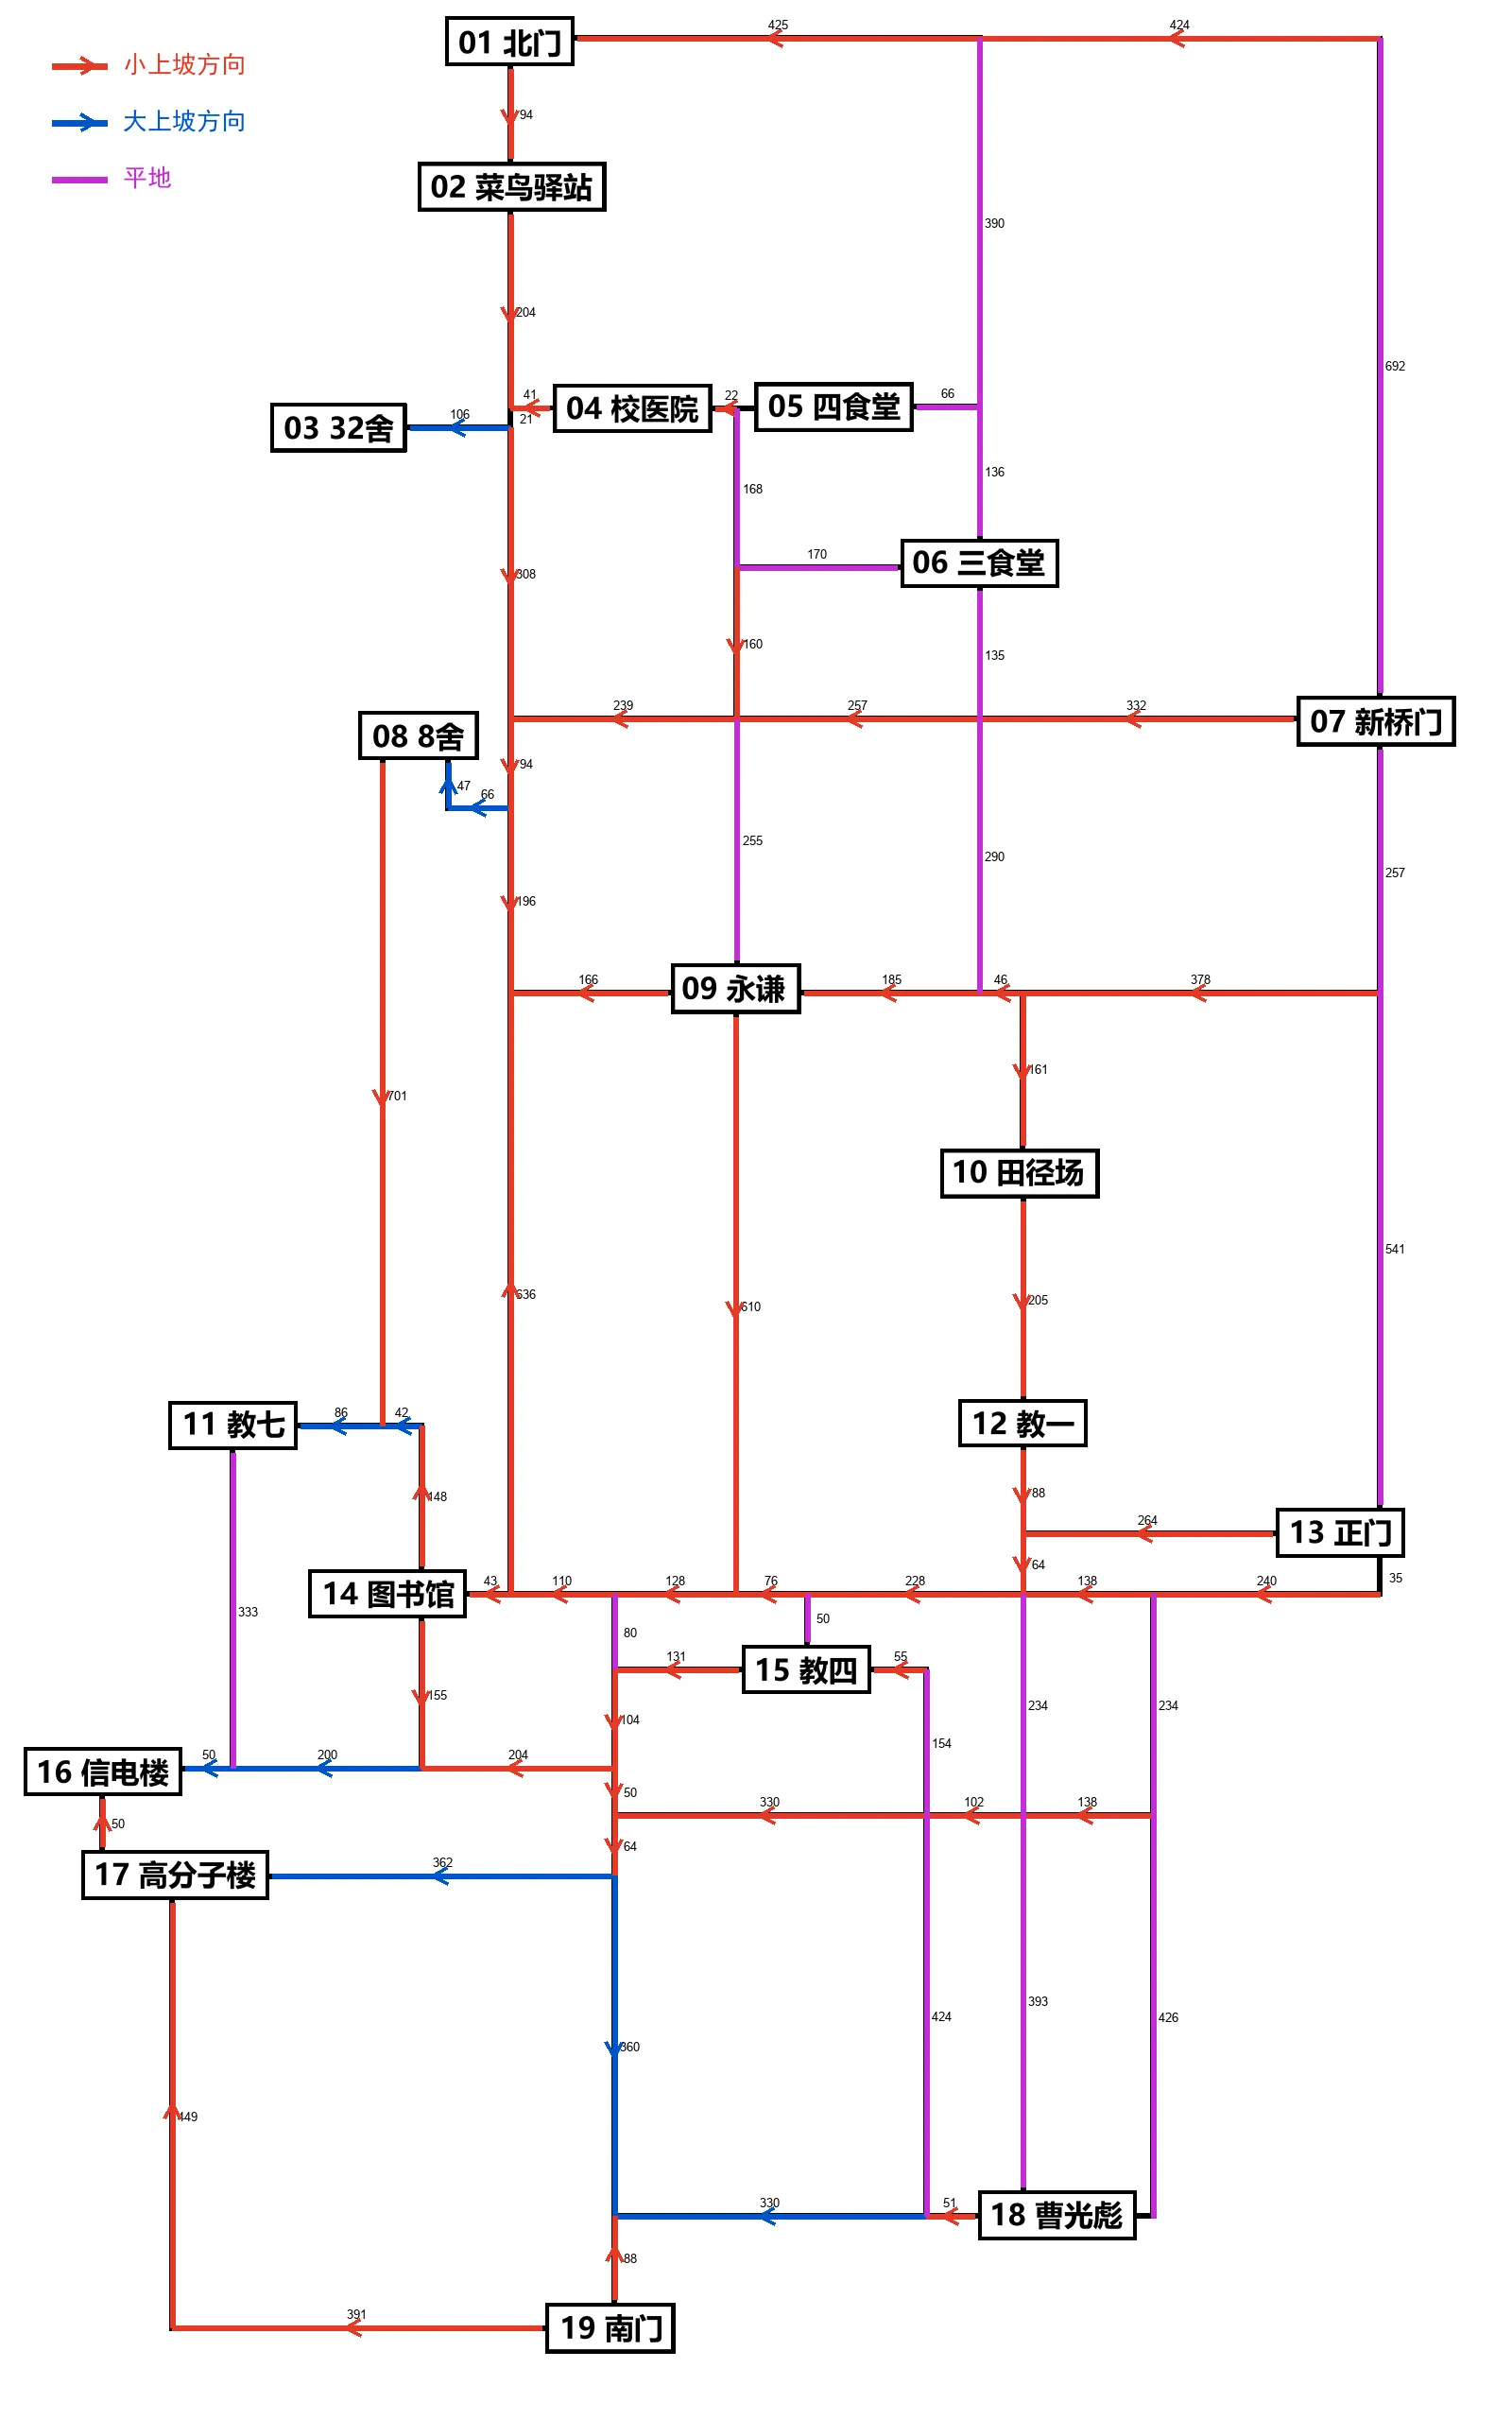
\includegraphics[width=0.75\textwidth]{figures/report_topology_final.png}
    \caption{玉泉校区简化道路拓扑图与坡度标注}
    \label{fig:topology}
\end{figure}

\section{综合时间代价模型}

\subsection{基础道路时间代价}

项目根据人工标定得到图上距离和实际距离的换算关系。由记录可知，从北门到校医院的图上距离约为 $94+204$ 个单位，对应实际距离约 200 米，因此：
\[
    1\ \text{图上距离单位} \approx \frac{200}{94+204} \approx 0.671\ \text{m}
\]

电瓶车基础速度取 25 km/h，即：
\[
    25\ \text{km/h} = 416.67\ \text{m/min}
\]

若某条边图上距离为 $d$，则基础行驶时间为：
\[
    time\_min = \frac{d \times 0.671}{416.67}
\]

坡度系数设置如下：
\[
\begin{array}{c|c}
\text{坡度类型} & \text{系数} \\
\hline
flat & 1.00 \\
slight\_up & 1.20 \\
steep\_up & 1.50 \\
slight\_down & 0.85 \\
steep\_down & 0.75 \\
\end{array}
\]

基础道路代价为：
\[
    base\_cost = time\_min \times slope\_factor
\]

\subsection{天气与货物重量情景代价}

天气和货物重量的影响并不是对整条路线统一放大，而是根据边的坡度类别逐边计算。系统首先将坡度类型归类为 flat、up、down：
\[
\begin{array}{c|c}
\text{原坡度类型} & \text{归类} \\
\hline
flat & flat \\
slight\_up, steep\_up & up \\
slight\_down, steep\_down & down \\
\end{array}
\]

情景边代价公式为：
\[
    context\_cost = base\_cost \times weather\_factor \times cargo\_factor
\]

天气规则如下：
\[
\begin{array}{c|ccc}
\text{天气} & flat & up & down \\
\hline
sunny & 1.00 & 1.00 & 1.00 \\
rainy & 1.25 & 1.00 & 1/0.6 \\
hot & 1/0.9 & 1/0.75 & 1.00 \\
\end{array}
\]

货物重量规则如下：
\[
\begin{array}{c|ccc}
\text{货物} & flat & up & down \\
\hline
small & 1.00 & 1.00 & 1.00 \\
medium & 1.00 & 1/0.8 & 1.00 \\
heavy & 1.00 & 2.00 & 1/0.8 \\
\end{array}
\]

项目根据 \texttt{data/context\_config.json} 中的当前情景配置，读取 \texttt{data/directed\_edges.csv} 并逐条边计算情景代价，输出 \texttt{data/context\_edges.csv}，随后重新运行 Dijkstra，生成 \texttt{data/context\_cost\_matrix.csv} 和 \texttt{data/context\_path\_matrix.json}。

\subsection{地点停留惩罚}

为了模拟校园跑腿配送中的非行驶时间，项目设置了特殊地点停留惩罚，配置文件为 \texttt{data/node\_delay.json}。当前规则如表 \ref{tab:delay} 所示。

\begin{table}[H]
\centering
\caption{特殊地点停留惩罚}
\label{tab:delay}
\begin{tabular}{c|c|c}
\hline
节点 & 地点 & 停留时间 \\
\hline
3 & 32舍 & 5 min \\
5 & 四食堂 & 2 min \\
6 & 三食堂 & 2 min \\
8 & 8舍 & 5 min \\
10 & 田径场 & 2 min \\
16 & 信电楼 & 1 min \\
19 & 南门 & 2 min \\
\hline
\end{tabular}
\end{table}

需要注意的是，停留惩罚不是只看最终配送点集合，而是根据完整经过路径判断。系统会通过 \texttt{context\_path\_matrix.json} 展开每一段最短路，若完整路径经过特殊地点，则触发对应停留时间。每个特殊地点在一条完整路线中最多只计算一次。

\section{Dijkstra 最短路预处理}

道路层最短路预处理由 \texttt{src/shortest\_path.py}、\texttt{src/generate\_matrix.py} 和 \texttt{src/context\_cost\_model.py} 完成。项目没有使用 \texttt{networkx} 等图算法库，而是自行实现了基于优先队列的 Dijkstra 算法。

单源 Dijkstra 的核心步骤为：
\begin{enumerate}[label=(\arabic*)]
    \item 根据有向边表构建邻接表；
    \item 将源点距离初始化为 0，其余节点距离视为无穷大；
    \item 使用优先队列反复取出当前距离最小的节点；
    \item 对该节点的所有出边进行松弛；
    \item 记录前驱节点，用于恢复最短路径。
\end{enumerate}

为了得到任意两点之间的最短路，系统对每个节点运行一次 Dijkstra，最终生成：
\begin{itemize}
    \item \texttt{cost\_matrix.csv}：基础任意两点最短行驶时间矩阵；
    \item \texttt{path\_matrix.json}：基础任意两点最短路径节点序列；
    \item \texttt{context\_cost\_matrix.csv}：当前情景下的最短行驶时间矩阵；
    \item \texttt{context\_path\_matrix.json}：当前情景下的最短路径节点序列。
\end{itemize}

预处理之后，配送顺序优化算法只需要查询矩阵，不必在每次评价路线时重新在道路图上运行最短路算法。

表 \ref{tab:dijkstra_preprocess_compare} 展示了预处理前后的差异。该设计的核心思想是将“道路层最短路问题”和“配送点访问顺序问题”分离：Dijkstra 负责在道路图上预先求出任意两点最短路，后续贪心、模拟退火和蚁群算法只需要在配送点集合上搜索访问顺序。

\begin{table}[H]
\centering
\caption{Dijkstra 预处理前后的路线评价方式对比}
\label{tab:dijkstra_preprocess_compare}
\small
\renewcommand{\arraystretch}{1.2}
\begin{tabularx}{\textwidth}{c|X|X}
\hline
方案 & 路线评价方式 & 特点 \\
\hline
不预处理 & 每次评价两个配送点之间的代价时重新运行 Dijkstra & 重复计算多，启发式算法大量评价候选路线时效率较低 \\
\hline
Dijkstra 预处理 & 直接查询 \texttt{context\_cost\_matrix.csv} & 任意两点行驶时间查询近似为 $O(1)$，适合反复评价路线 \\
\hline
路径展开 & 查询 \texttt{context\_path\_matrix.json} & 获得两点最短路完整节点序列，用于判断是否触发地点停留惩罚 \\
\hline
\end{tabularx}
\end{table}

下面给出 Dijkstra 中最关键的“取最小距离节点 + 松弛出边”代码片段。可以看到，算法只依赖邻接表和优先队列，不调用现成图算法库：

\begin{lstlisting}[caption={Dijkstra 核心松弛过程}]
while heap:
    cur_dist, u = heapq.heappop(heap)
    if cur_dist > dist[u]:
        continue

    for v, weight in graph[u]:
        new_dist = cur_dist + weight
        if new_dist < dist[v]:
            dist[v] = new_dist
            prev[v] = u
            heapq.heappush(heap, (new_dist, v))
\end{lstlisting}

\section{配送路径优化算法设计}

道路层最短路已经由 Dijkstra 预处理完成，因此本节算法优化的不是地图上的单源最短路，而是多个配送点的访问顺序。三种启发式算法和精确 DP 的定位如表 \ref{tab:algorithm_overview} 所示。它们统一使用
\[
    total\_time = drive\_time + delay\_time
\]
作为评价标准，其中 \texttt{drive\_time} 来自当前情景下的最短路矩阵，\texttt{delay\_time} 来自完整路径中触发的地点停留惩罚。

\begin{table}[H]
\centering
\caption{路径优化算法在本项目中的作用}
\label{tab:algorithm_overview}
\small
\renewcommand{\arraystretch}{1.2}
\begin{tabularx}{\textwidth}{c|X|X|X|X}
\hline
算法 & 本项目中的作用 & 搜索方式 & 优点 & 局限 \\
\hline
贪心 & baseline，快速生成初始配送顺序 & 每一步选择当前增量 \texttt{total\_time} 最小的配送点 & 速度最快，结果稳定，便于对比 & 只看局部选择，可能错过全局更优顺序 \\
\hline
模拟退火 & 在贪心路线基础上继续优化 & 对配送顺序做 swap/reverse，并用 Metropolis 准则接受新解 & 能跳出局部最优，通常优于贪心 & 结果受温度、迭代次数和随机种子影响 \\
\hline
蚁群算法 & 多路径群体搜索配送顺序 & 信息素 $\tau$ 与启发函数 $\eta=1/cost$ 共同决定转移概率 & 全局搜索能力较强，适合多点组合优化 & 运行时间较长，参数较多 \\
\hline
精确 DP & 小规模任务最优性验证 & 状态压缩枚举访问集合、当前位置和已触发停留点集合 & 可证明当前模型下全局最优 & 状态数指数增长，不适合大规模任务 \\
\hline
\end{tabularx}
\end{table}

\subsection{最近邻贪心算法}

最近邻贪心算法实现于 \texttt{src/algorithms/greedy.py}。算法从起点出发，每一步在尚未访问的配送点中选择当前增量总代价最小的点，直到访问完所有配送点。

这里的增量总代价不是单纯的行驶时间，而是：
\[
    segment\_total\_cost(i,j)
    = drive\_time(i,j) + new\_delay(i,j)
\]
其中，$new\_delay(i,j)$ 表示从当前点 $i$ 到候选点 $j$ 的最短路径中新触发的停留惩罚。这样可以避免算法只看距离而忽略经过食堂、宿舍等地点造成的时间增加。

贪心算法的核心选择过程如下。每一步都枚举尚未访问的配送点，选出当前增量总代价最小的候选点：

\begin{lstlisting}[caption={最近邻贪心的候选点选择}]
while unvisited:
    best_point = None
    best_delta = float("inf")

    for candidate in unvisited:
        delta = segment_total_cost(
            current, candidate, cost_lookup,
            path_matrix, node_delay, delayed_nodes
        )
        if delta < best_delta:
            best_delta = delta
            best_point = candidate

    route.append(best_point)
    current = best_point
    unvisited.remove(best_point)
\end{lstlisting}

贪心算法的优点是实现简单、运行速度快，适合在 UI 中快速给出 baseline 结果；缺点是只做局部最优选择，不保证全局最优。

\subsection{模拟退火算法}

模拟退火算法实现于 \texttt{src/algorithms/simulated\_annealing.py}。算法使用考虑停留惩罚的贪心路线作为初始解，然后通过随机邻域操作搜索更优路线。邻域操作包括：
\begin{itemize}
    \item \textbf{swap}：交换两个配送点的访问顺序；
    \item \textbf{reverse}：反转一段配送点序列。
\end{itemize}

起点不参与邻域交换。对于新生成的候选路线，若总代价更低则直接接受；若总代价更高，则以 Metropolis 准则接受：
\[
    P=\exp\left(-\frac{new\_cost-old\_cost}{T}\right)
\]
其中 $T$ 为当前温度。温度按照
\[
    T = T \times \alpha
\]
逐步下降。当前默认参数为：
\begin{verbatim}
initial_temp = 10.0
final_temp = 1e-4
alpha = 0.95
inner_iter = 100
seed = 42
\end{verbatim}

模拟退火的关键在于接受准则。下面代码体现了“更优解必然接受，更差解按概率接受”的思想：

\begin{lstlisting}[caption={模拟退火 Metropolis 接受准则}]
delta = new_cost - current_cost

if delta <= 0:
    accept = True
else:
    accept_prob = math.exp(-delta / temperature)
    accept = random.random() < accept_prob

if accept:
    current_route = new_route
    current_cost = new_cost

if current_cost < best_cost:
    best_route = current_route[:]
    best_cost = current_cost
\end{lstlisting}

模拟退火算法通过概率接受较差解，具有跳出局部最优的能力，但结果会受到参数和随机种子的影响。

\subsection{蚁群算法}

蚁群算法实现于 \texttt{src/algorithms/ant\_colony.py}。每只蚂蚁从指定起点出发，根据当前点到候选配送点之间的信息素和启发函数，概率选择下一个配送点。转移概率为：
\[
    p(i,j) \propto \tau(i,j)^\alpha \cdot \eta(i,j)^\beta
\]
其中，$\tau(i,j)$ 为信息素强度，$\eta(i,j)$ 为启发函数。当前项目中启发函数定义为：
\[
    \eta(i,j)=\frac{1}{segment\_total\_cost(i,j)}
\]
因此，距离近且新增停留惩罚较小的候选点更容易被选择。

每轮所有蚂蚁完成路线构造后，信息素统一挥发：
\[
    \tau = \tau \times (1-\rho)
\]
并根据路线总代价增加信息素：
\[
    \Delta\tau \propto \frac{1}{total\_time}
\]
路线越优，增加的信息素越多。当前默认参数为：
\begin{verbatim}
num_ants = 30
num_iterations = 100
alpha = 1.0
beta = 3.0
rho = 0.3
q = 1.0
seed = 42
\end{verbatim}

蚁群算法中，下一个配送点不是固定选择最短边，而是根据“信息素 + 启发函数”计算概率后随机选择：

\begin{lstlisting}[caption={蚁群算法的转移概率计算}]
weights = []
for candidate in unvisited:
    cost = segment_total_cost(current, candidate, cost_lookup,
                              path_matrix, node_delay, delayed_nodes)
    eta = 1.0 / cost
    score = (tau[current, candidate] ** alpha) * (eta ** beta)
    weights.append((candidate, score))

next_point = roulette_wheel_select(weights)
\end{lstlisting}

\subsection{状态压缩 DP 精确对照}

贪心、模拟退火和蚁群算法都属于启发式算法，不能保证一定得到全局最优解。为了验证小规模任务中的解质量，项目实现了状态压缩动态规划精确对照算法，相关文件为 \texttt{src/algorithms/exact\_dp.py} 和 \texttt{src/exact\_dp\_context.py}。

由于本项目的总代价包含“每个特殊地点最多触发一次”的停留惩罚，DP 状态不仅需要记录已经访问的配送点集合，还需要记录已经触发过的停留节点集合。状态可表示为：
\[
    (visited\_mask,\ last,\ delay\_mask)
\]
其中，\verb|visited_mask| 表示已经访问的配送点集合，\verb|last| 表示当前所在配送点，\verb|delay_mask| 表示已经触发过的特殊停留节点集合。

状态转移为：从当前状态选择一个尚未访问的配送点，查询当前点到该点的情景最短路行驶时间，并根据展开路径更新新增停留惩罚。每个状态只保留当前已知的最小总代价。因此，当所有配送点均被访问后，DP 得到的是当前模型下的小规模精确最优解。

状态压缩 DP 的核心转移代码如下。由于它枚举了所有访问集合和最后所在节点，所以在小规模任务下可以作为精确最优解对照：

\begin{lstlisting}[caption={状态压缩 DP 的核心状态转移}]
for state, cur_cost in dp.items():
    visited_mask, last, delay_mask = state

    for nxt in delivery_points:
        bit = point_bit[nxt]
        if visited_mask & bit:
            continue

        drive = cost_lookup[last, nxt]
        extra_delay, new_delay_mask = calc_extra_delay(
            last, nxt, delay_mask, path_matrix, node_delay
        )

        new_state = (visited_mask | bit, nxt, new_delay_mask)
        new_cost = cur_cost + drive + extra_delay
        if new_cost < dp.get(new_state, float("inf")):
            dp[new_state] = new_cost
            parent[new_state] = state
\end{lstlisting}

\newpage
\section{系统实现}

当前项目的核心代码结构如下：
\begin{verbatim}
src/
├── build_graph.py
├── generate_matrix.py
├── shortest_path.py
├── context_cost_model.py
├── route_common.py
├── visualize_route_animation.py
├── exact_dp_context.py
├── algorithms/
│   ├── greedy.py
│   ├── simulated_annealing.py
│   ├── ant_colony.py
│   └── exact_dp.py
├── interface/
│   └── planner_ui.py
└── visualization/
    └── visualize_route_animation.py
\end{verbatim}

其中，\texttt{route\_common.py} 负责路线代价计算、路径展开、停留惩罚和 CSV 读写；\texttt{context\_cost\_model.py} 负责天气和货物情景代价矩阵生成；\texttt{interface/planner\_ui.py} 为最终交互入口。运行方式为：
\begin{verbatim}
python src/interface/planner_ui.py
\end{verbatim}

UI 支持选择起点、配送点、是否回到起点、天气、货物重量和算法类型。若算法选择为 all，则系统会同时运行贪心、模拟退火和蚁群算法，并按总时间选择推荐路线。系统还会输出 \texttt{results/interactive\_result.csv} 和 \texttt{results/algorithm\_comparison\_context.csv}。

\newpage
\section{实验结果与分析}

当前项目结果文件显示，测试情景为 sunny + small，起点为北门，配送任务包含菜鸟驿站、32舍、三食堂、新桥门、图书馆、南门等地点，且不要求回到起点。三种算法对比结果如表 \ref{tab:comparison} 所示。

\begin{table}[H]
\centering
\caption{三种算法路线结果对比}
\label{tab:comparison}
\small
\begin{tabularx}{\textwidth}{c|X|c|c|c}
\hline
算法 & 路线 & 行驶时间/min & 停留时间/min & 总时间/min \\
\hline
greedy & 北门 $\rightarrow$ 菜鸟驿站 $\rightarrow$ 图书馆 $\rightarrow$ 新桥门 $\rightarrow$ 三食堂 $\rightarrow$ 32舍 $\rightarrow$ 南门 & 10.79 & 9.00 & 19.79 \\
\hline
simulated\_annealing & 北门 $\rightarrow$ 菜鸟驿站 $\rightarrow$ 32舍 $\rightarrow$ 三食堂 $\rightarrow$ 新桥门 $\rightarrow$ 图书馆 $\rightarrow$ 南门 & 6.83 & 9.00 & 15.83 \\
\hline
ant\_colony & 北门 $\rightarrow$ 菜鸟驿站 $\rightarrow$ 32舍 $\rightarrow$ 三食堂 $\rightarrow$ 新桥门 $\rightarrow$ 图书馆 $\rightarrow$ 南门 & 6.83 & 9.00 & 15.83 \\
\hline
\end{tabularx}
\end{table}

从结果可以看出，贪心算法由于每一步只选择当前局部增量最小的配送点，最终路线行驶时间为 10.79 分钟，总时间为 19.79 分钟。模拟退火和蚁群算法通过全局搜索或群体搜索找到了更优访问顺序，行驶时间降至 6.83 分钟，总时间为 15.83 分钟。

该实验体现了三类启发式算法的典型差异：贪心算法响应最快，可以作为 baseline；模拟退火和蚁群算法需要更多搜索时间，但能够通过调整访问顺序降低总配送时间。因此，在实际系统中可以同时运行三种算法，并按 \texttt{total\_time} 最小原则自动推荐路线。


\subsection{天气变化对路线的影响}

实验记录中还对不同天气情景下的路线变化进行了观察。由于本项目的天气系数不是对整条路线统一放大，而是分别作用于平地、上坡和下坡道路，因此天气变化会改变道路边权，进而可能改变两点之间的最短路和最终配送访问顺序。

在配送点较多、可选道路较复杂时，晴天、下雨天和大热天的路线可能出现明显差异。其原因是：下雨天对下坡边的惩罚较大，系统会倾向于避开部分下坡风险较高的路径；大热天对上坡边的惩罚较大，路线可能减少连续上坡路段；而晴天没有额外天气惩罚，路线更接近基础坡度时间下的结果。图 \ref{fig:weather_complex_sunny}--图 \ref{fig:weather_complex_hot} 分别展示了同一复杂任务在三种天气下得到的路线图。

\begin{figure}[H]
    \centering
    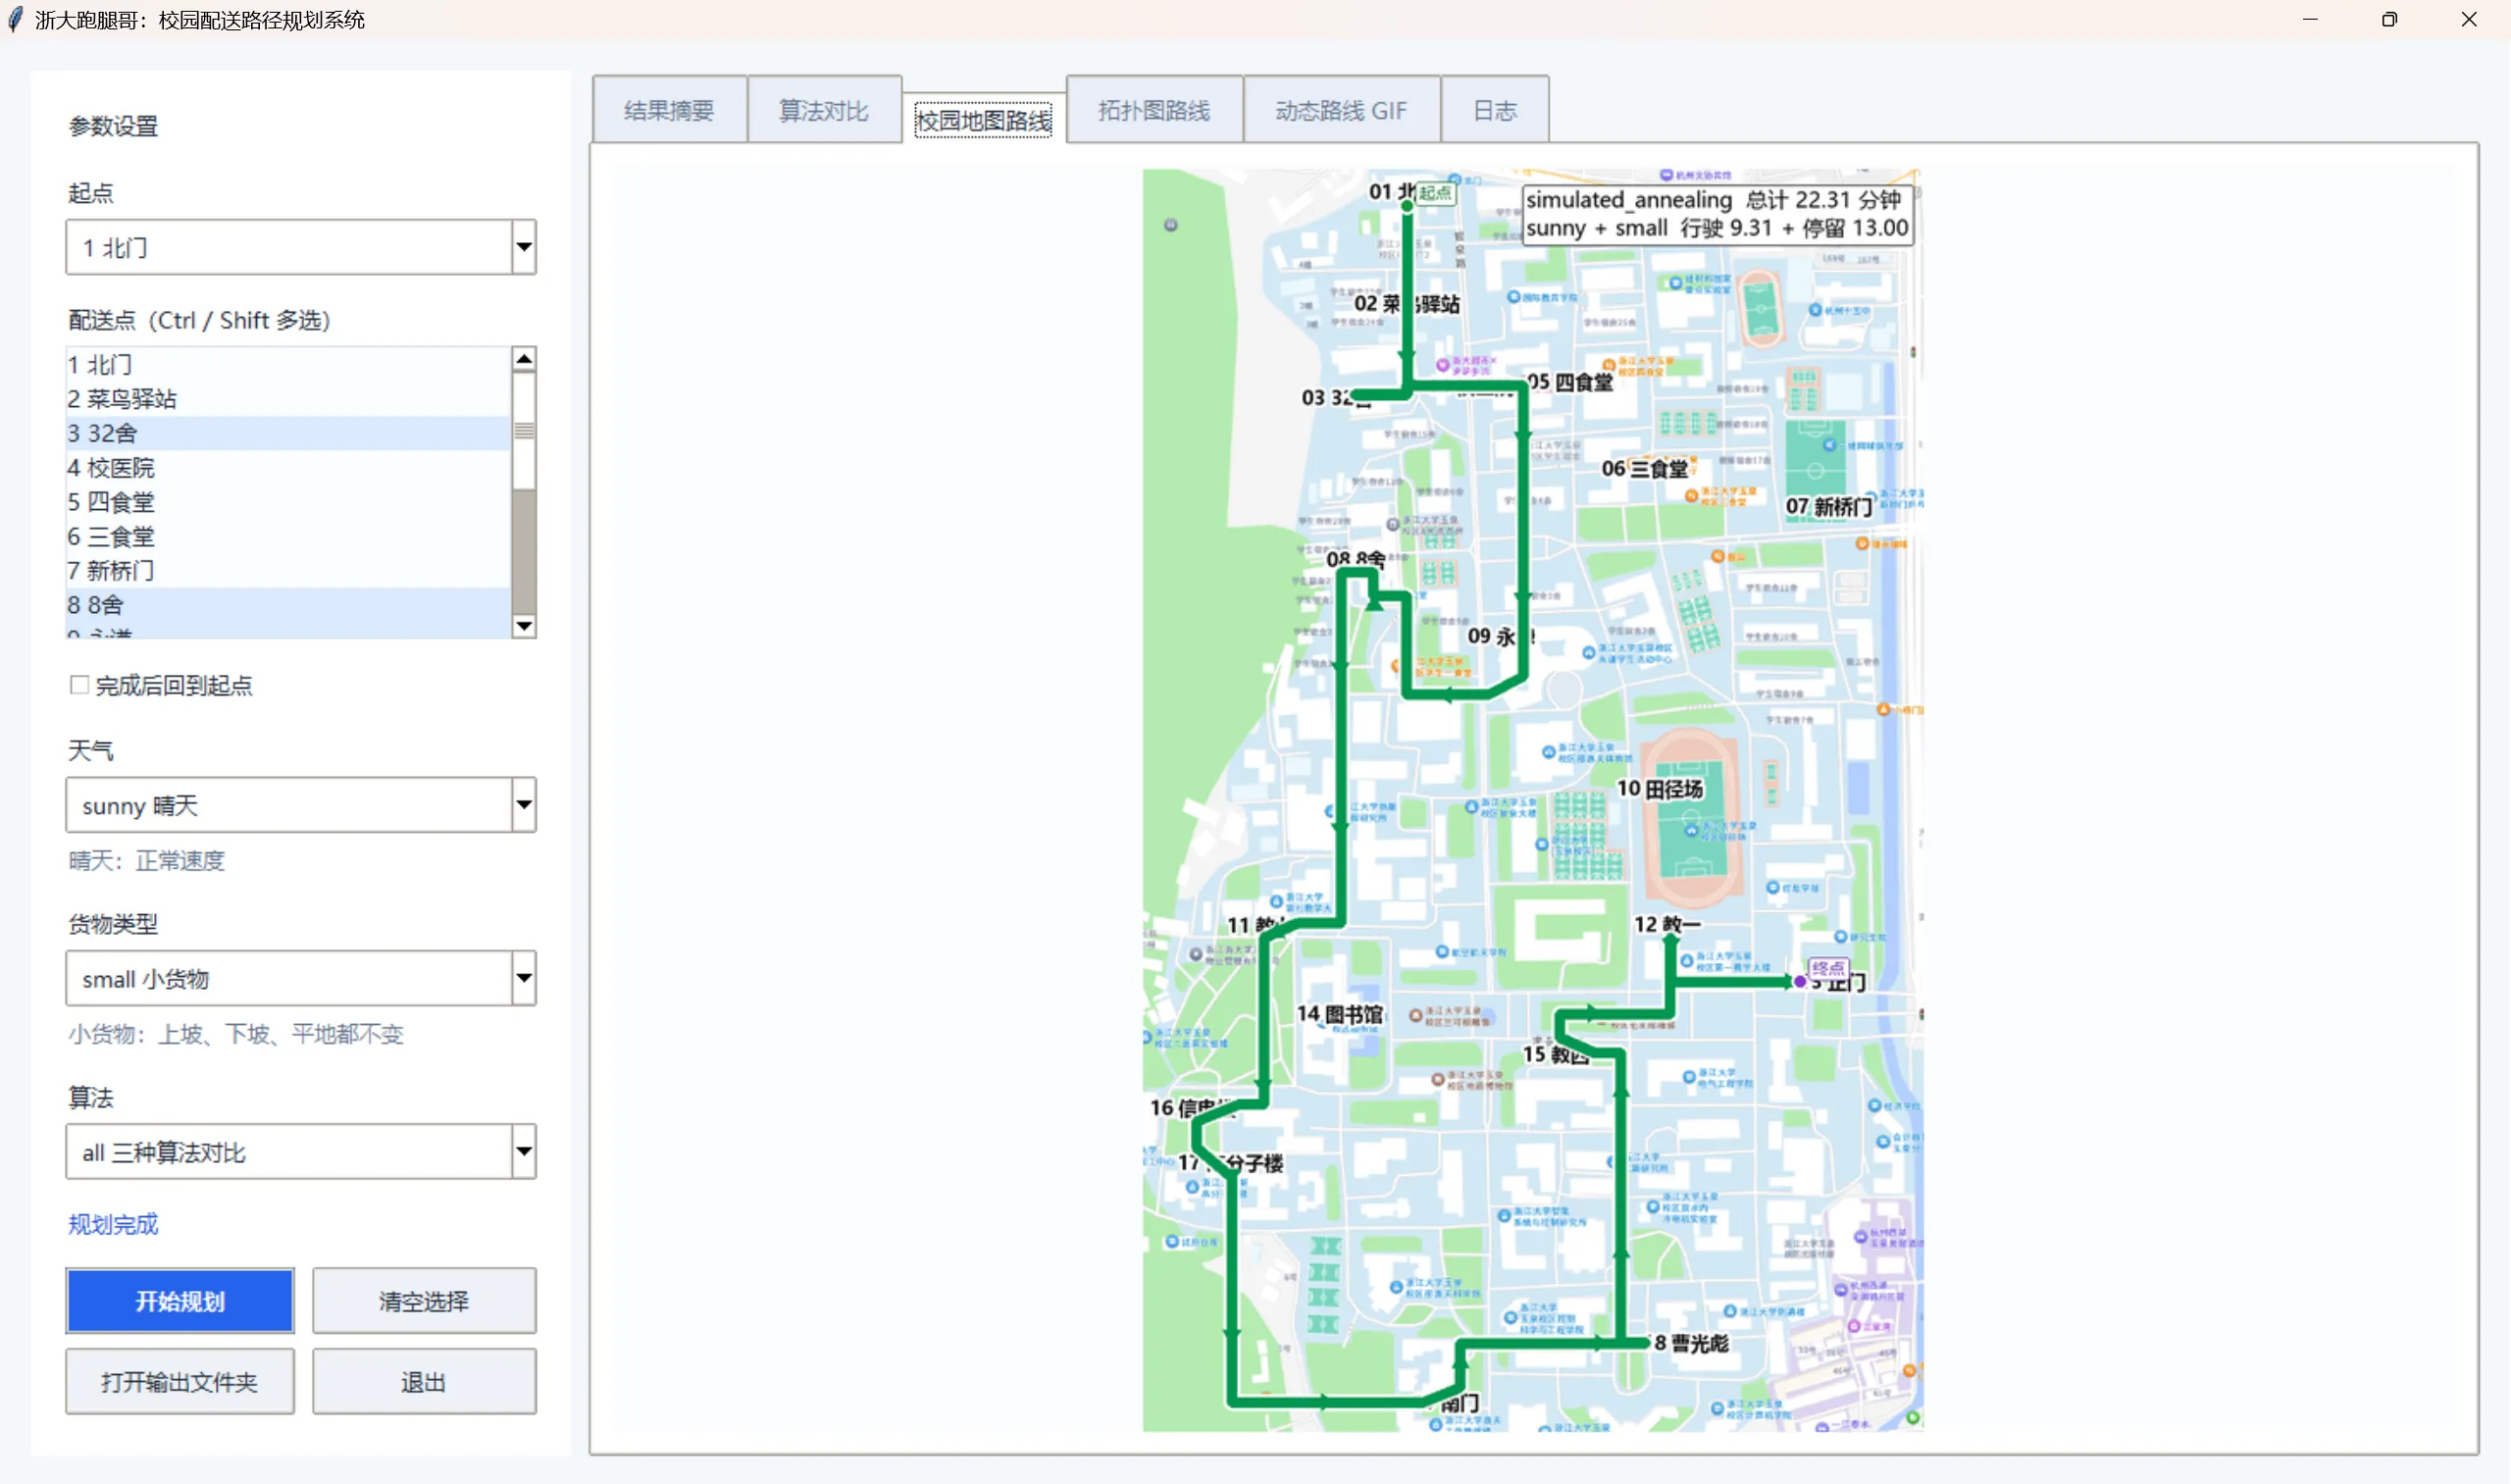
\includegraphics[width=0.92\textwidth]{figures/report_weather_complex_sunny_route.png}
    \caption{复杂配送任务在晴天 + 小货物情景下的路线}
    \label{fig:weather_complex_sunny}
\end{figure}

\begin{figure}[H]
    \centering
    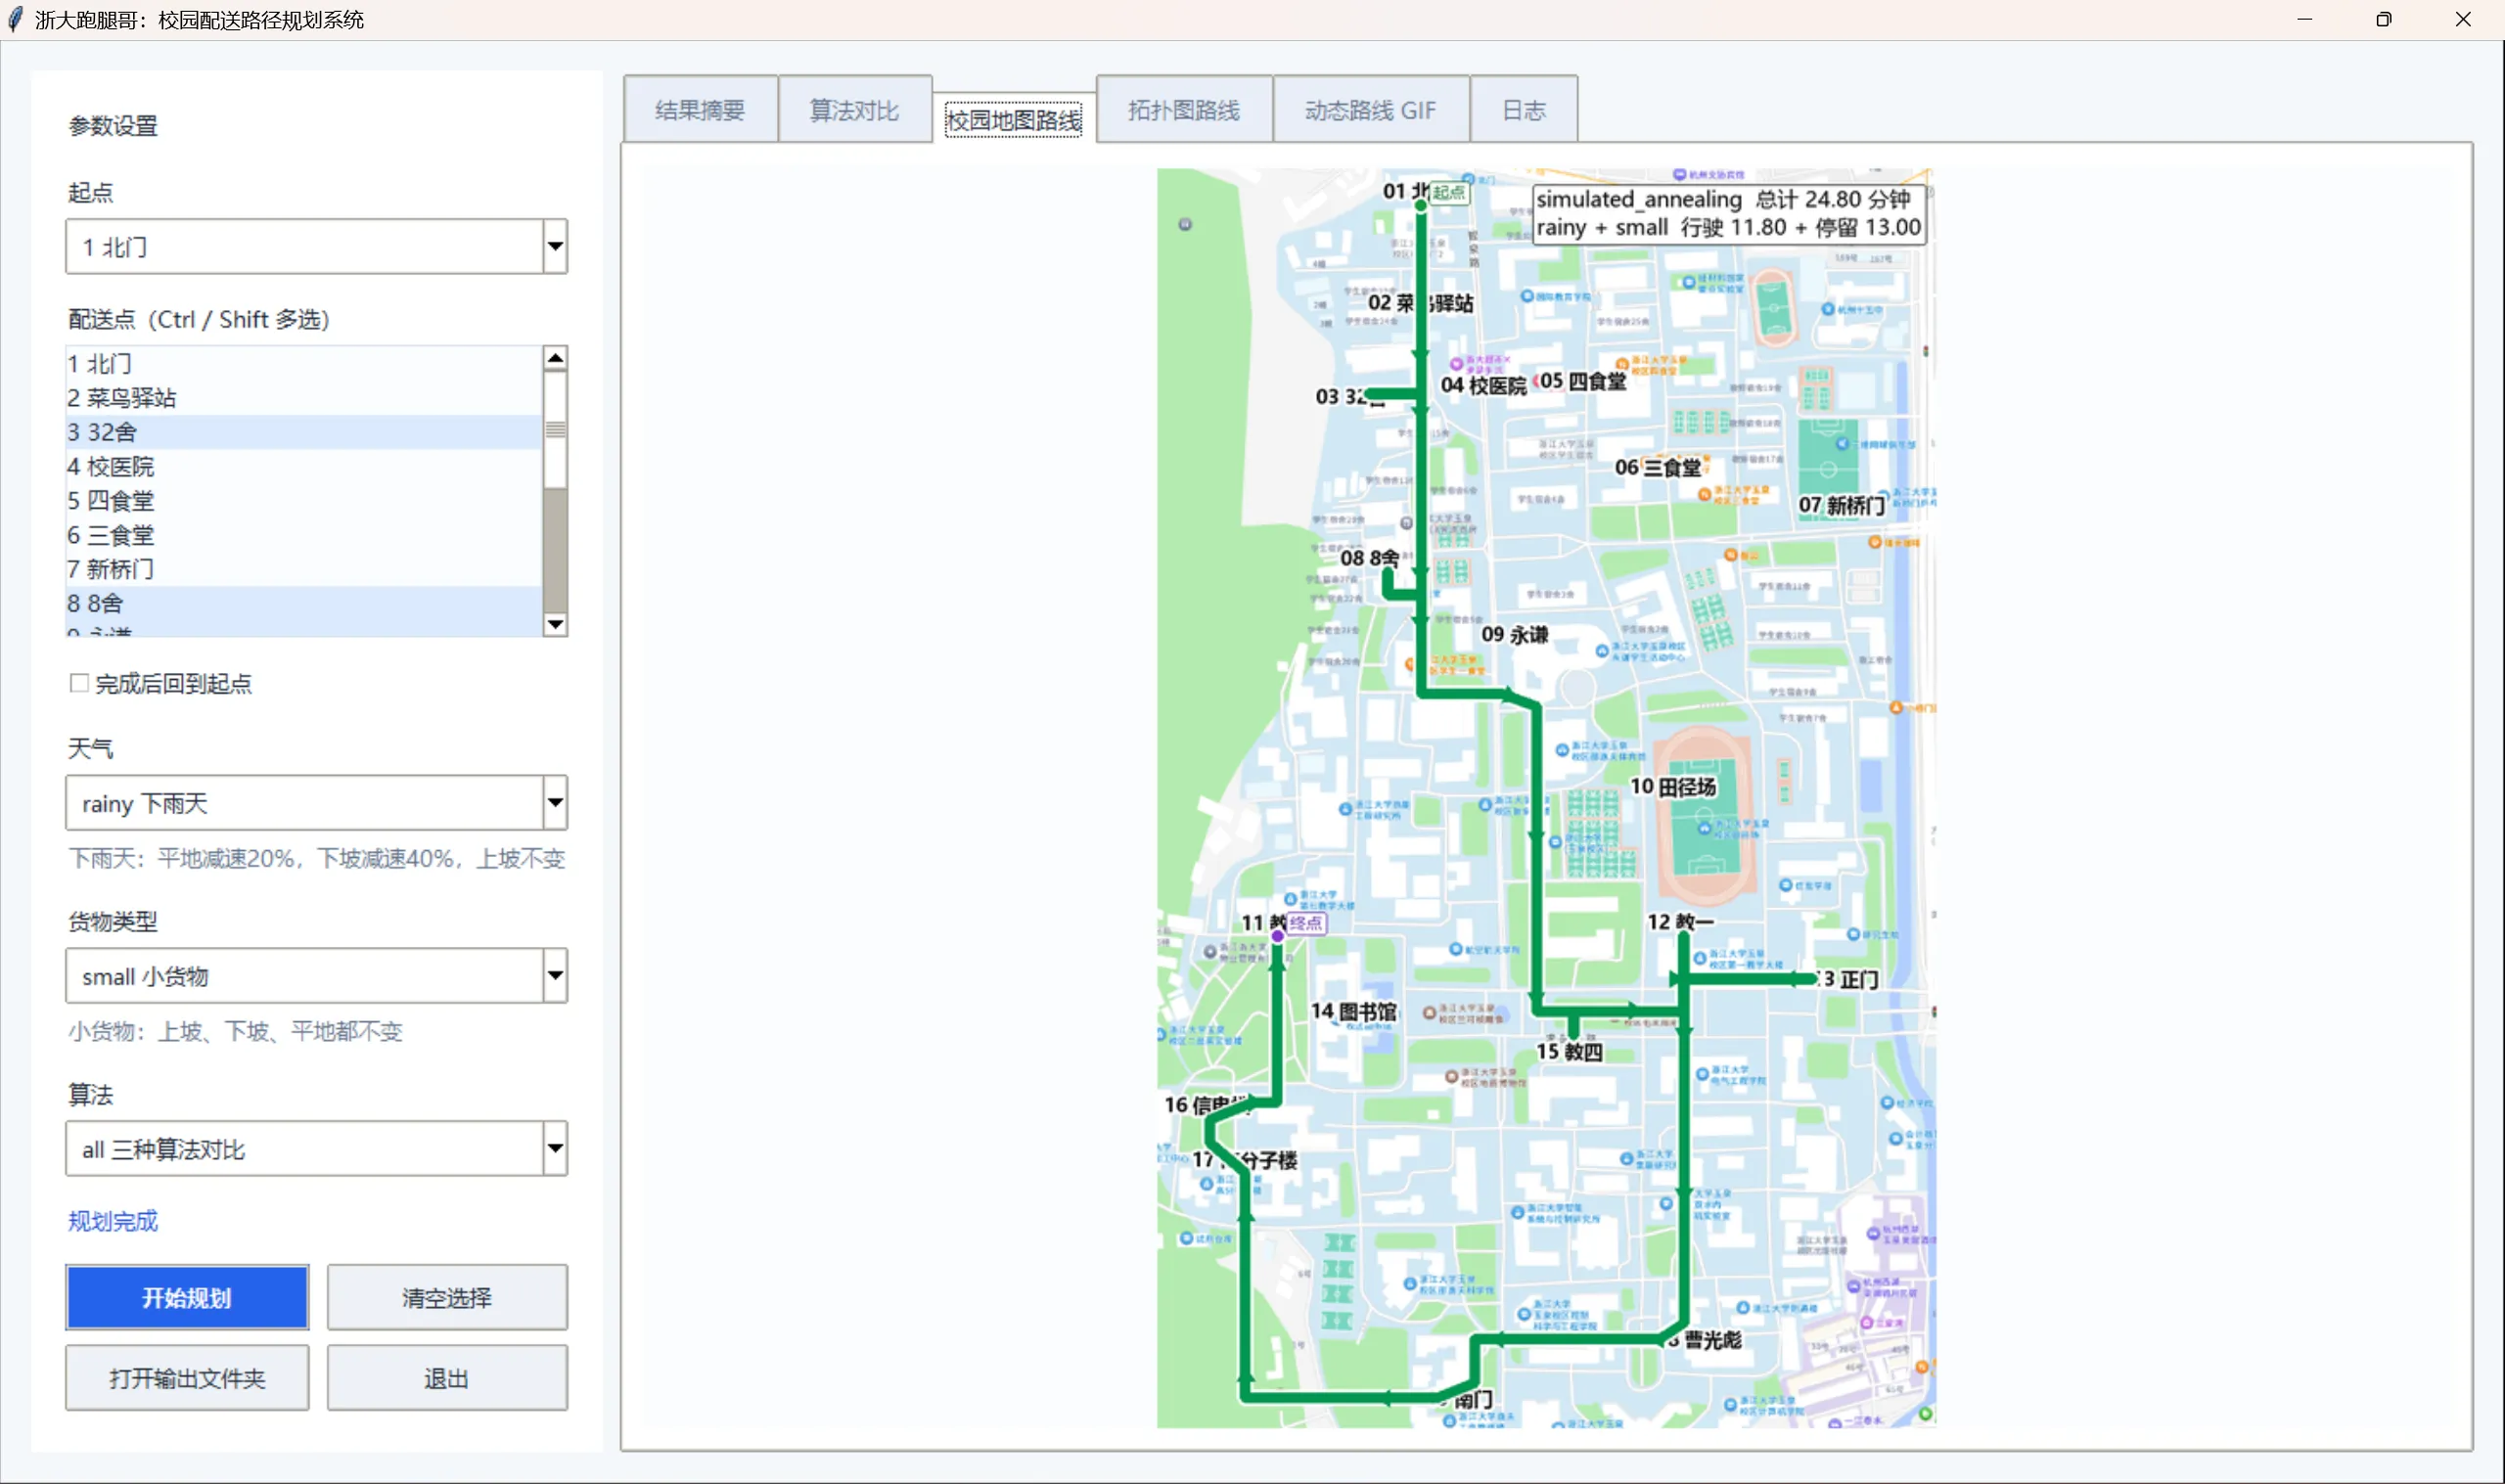
\includegraphics[width=0.92\textwidth]{figures/report_weather_complex_rainy_route.png}
    \caption{复杂配送任务在下雨天 + 小货物情景下的路线}
    \label{fig:weather_complex_rainy}
\end{figure}

\begin{figure}[H]
    \centering
    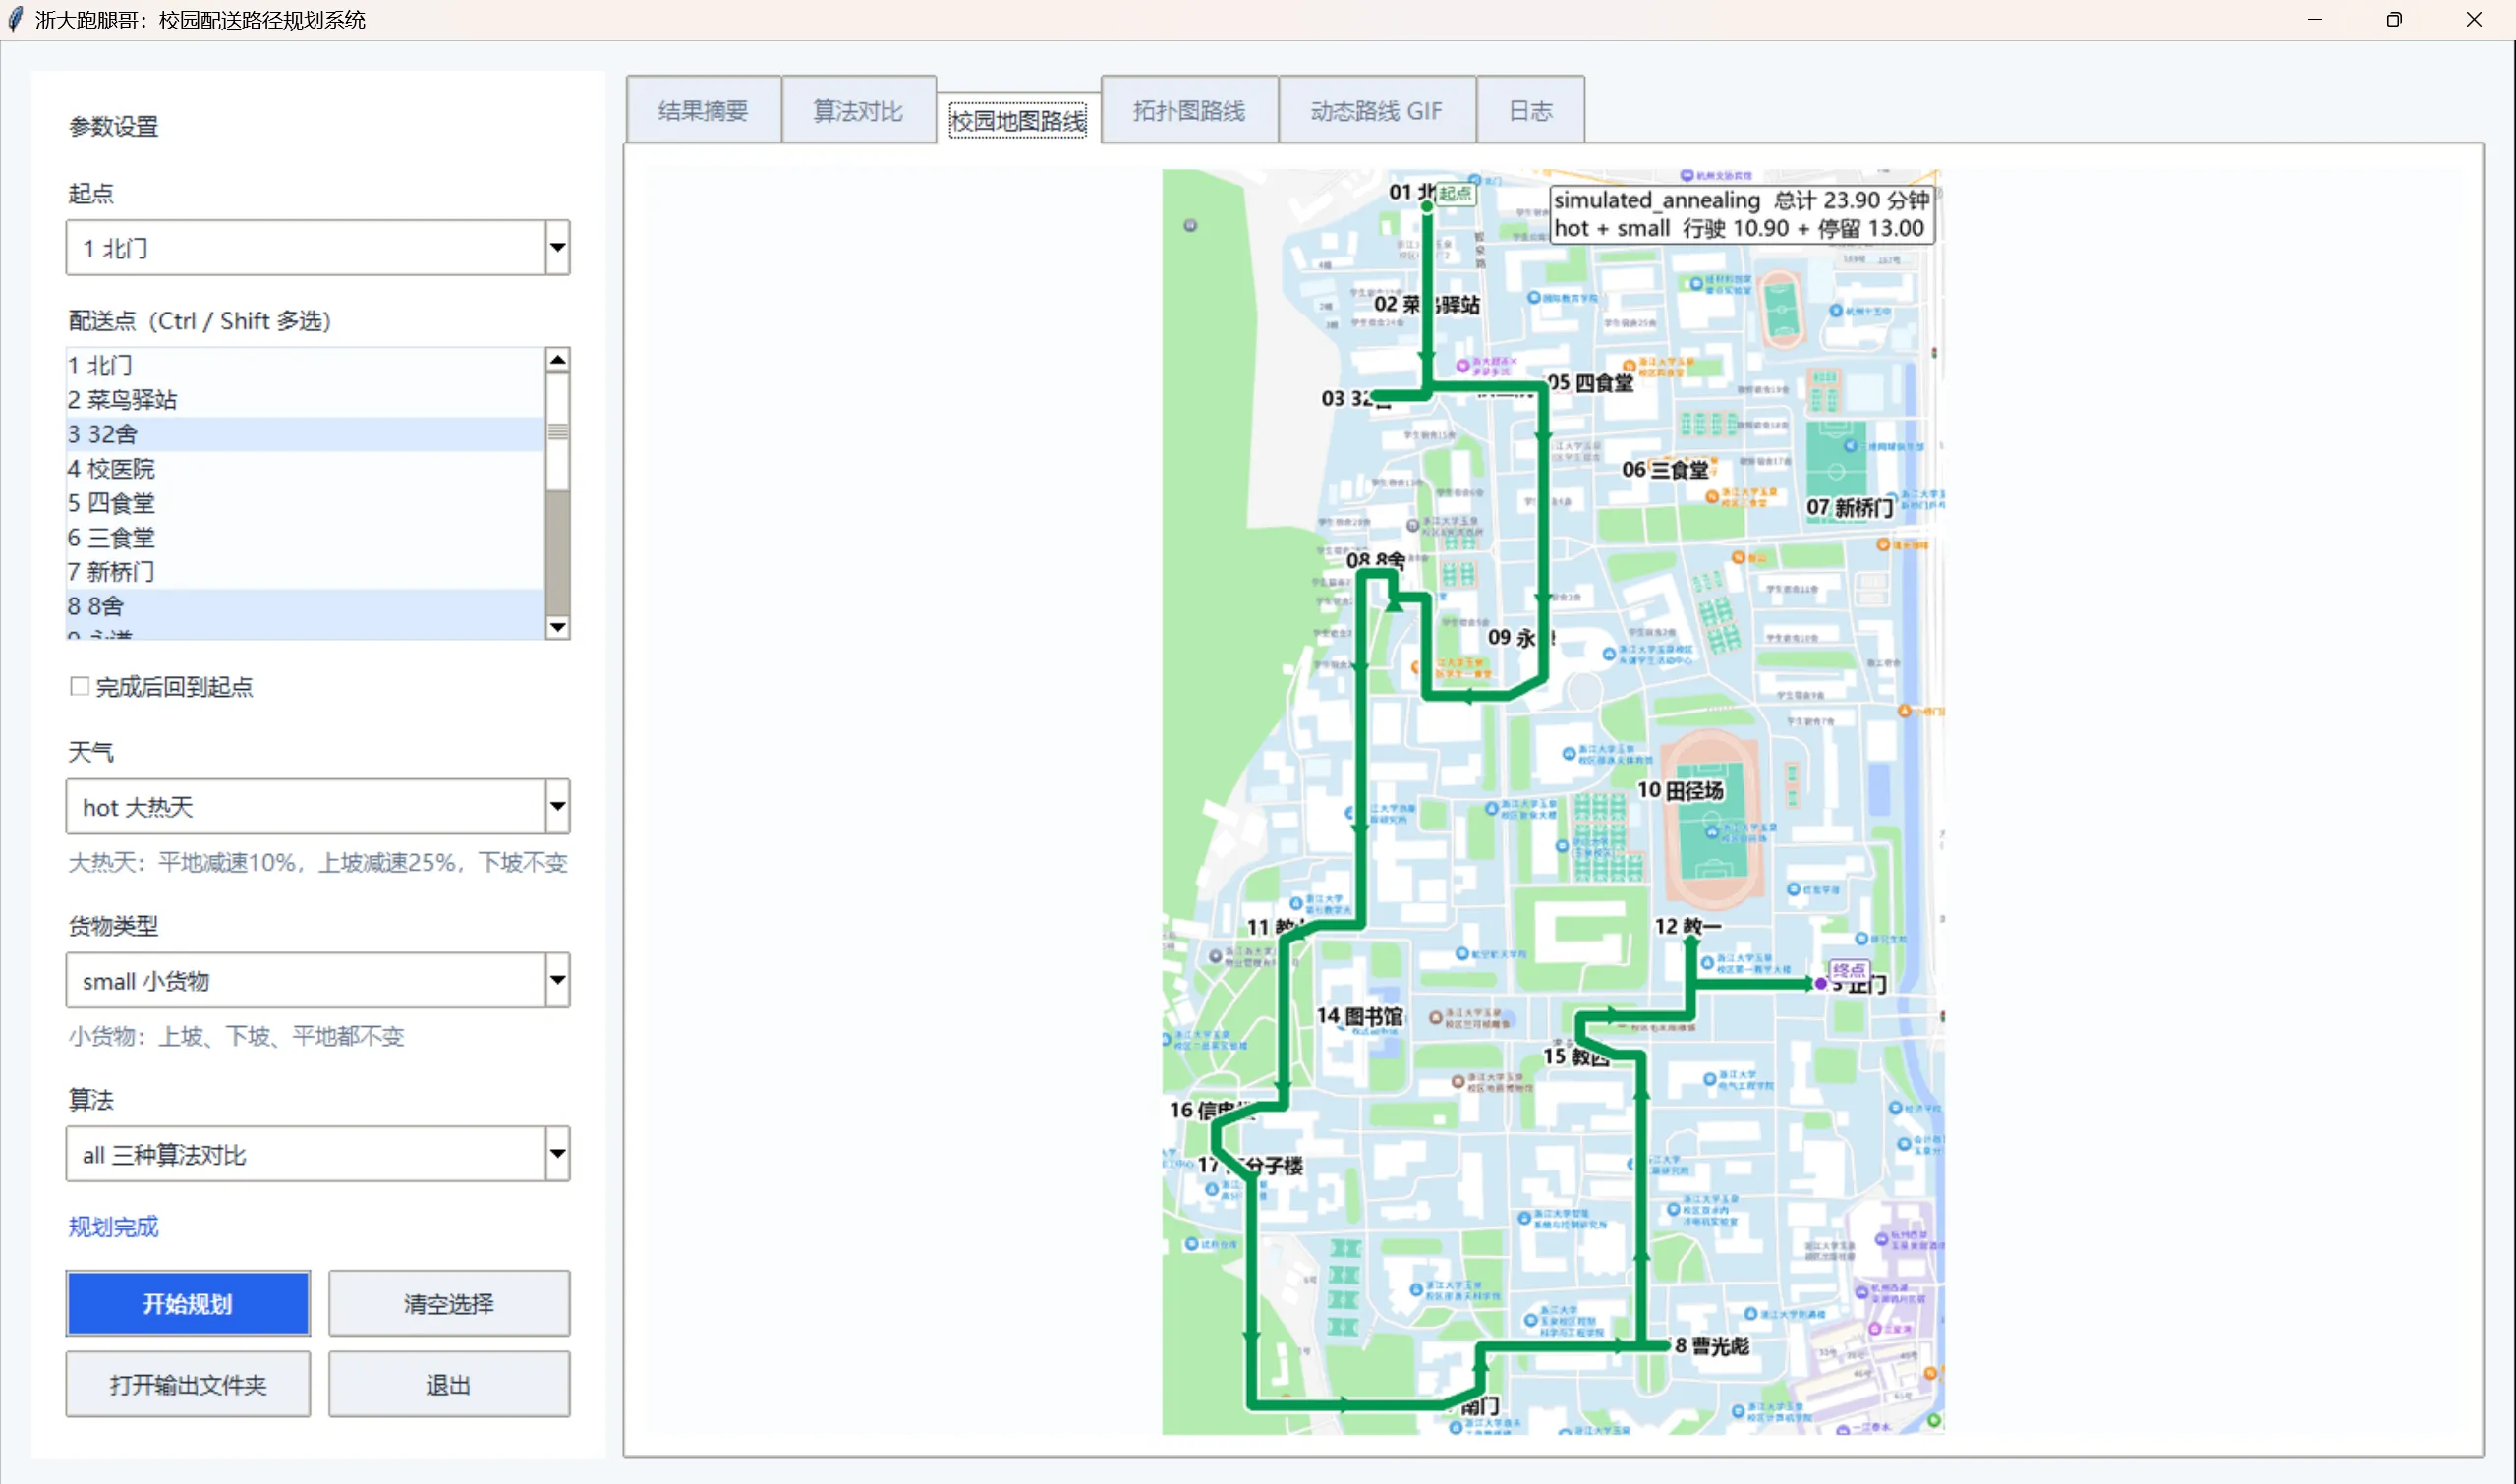
\includegraphics[width=0.92\textwidth]{figures/report_weather_complex_hot_route.png}
    \caption{复杂配送任务在大热天 + 小货物情景下的路线}
    \label{fig:weather_complex_hot}
\end{figure}


\begin{table}[H]
\centering
\caption{复杂配送任务中不同天气下的推荐路线数据}
\label{tab:weather_complex_summary}
\small
\renewcommand{\arraystretch}{1.2}
\begin{tabular}{c|c|c|c|c|c}
\hline
天气 & 货物 & 推荐算法 & 行驶时间/min & 停留时间/min & 总时间/min \\
\hline
晴天 & 小货物 & Simulated Annealing & 9.31 & 13.00 & 22.31 \\
\hline
下雨天 & 小货物 & Simulated Annealing & 11.80 & 13.00 & 24.80 \\
\hline
大热天 & 小货物 & Simulated Annealing & 10.90 & 13.00 & 23.90 \\
\hline
\end{tabular}
\end{table}


\begin{table}[H]
\centering
\caption{复杂配送任务中不同天气下的推荐路线}
\label{tab:weather_complex_routes}
\small
\renewcommand{\arraystretch}{1.25}
\begin{tabularx}{\textwidth}{c|>{\raggedright\arraybackslash}X}
\hline
天气 & 推荐路线 \\
\hline
晴天 &
北门 $\rightarrow$ 菜鸟驿站 $\rightarrow$ 32舍 $\rightarrow$ 8舍 $\rightarrow$ 永谦 $\rightarrow$ 教七 $\rightarrow$ 信电楼 $\rightarrow$ 高分子楼 $\rightarrow$ 南门 $\rightarrow$ 曹光彪 $\rightarrow$ 教四 $\rightarrow$ 教一 $\rightarrow$ 正门 \\
\hline
下雨天 &
北门 $\rightarrow$ 32舍 $\rightarrow$ 8舍 $\rightarrow$ 永谦 $\rightarrow$ 教四 $\rightarrow$ 教一 $\rightarrow$ 正门 $\rightarrow$ 曹光彪 $\rightarrow$ 南门 $\rightarrow$ 高分子楼 $\rightarrow$ 信电楼 \\
\hline
大热天 &
北门 $\rightarrow$ 32舍 $\rightarrow$ 永谦 $\rightarrow$ 8舍 $\rightarrow$ 教七 $\rightarrow$ 信电楼 $\rightarrow$ 高分子楼 $\rightarrow$ 南门 \\
\hline
\end{tabularx}
\end{table}



从表 \ref{tab:weather_complex_summary} 可以看出，天气变化不仅会改变路线图上的具体经过道路，也可能影响推荐算法得到的总时间。由于天气因子直接作用于每条有向边，路线变化并不是简单的整体时间放大，而是由局部边权变化累积后产生的结果。

为了进一步比较不同算法在复杂天气情景下的表现，项目分别记录了下雨天和大热天情景中的三算法运行结果。图 \ref{fig:rainy_algo_compare} 和图 \ref{fig:hot_algo_compare} 分别展示对应的界面结果。

\begin{figure}[H]
    \centering
    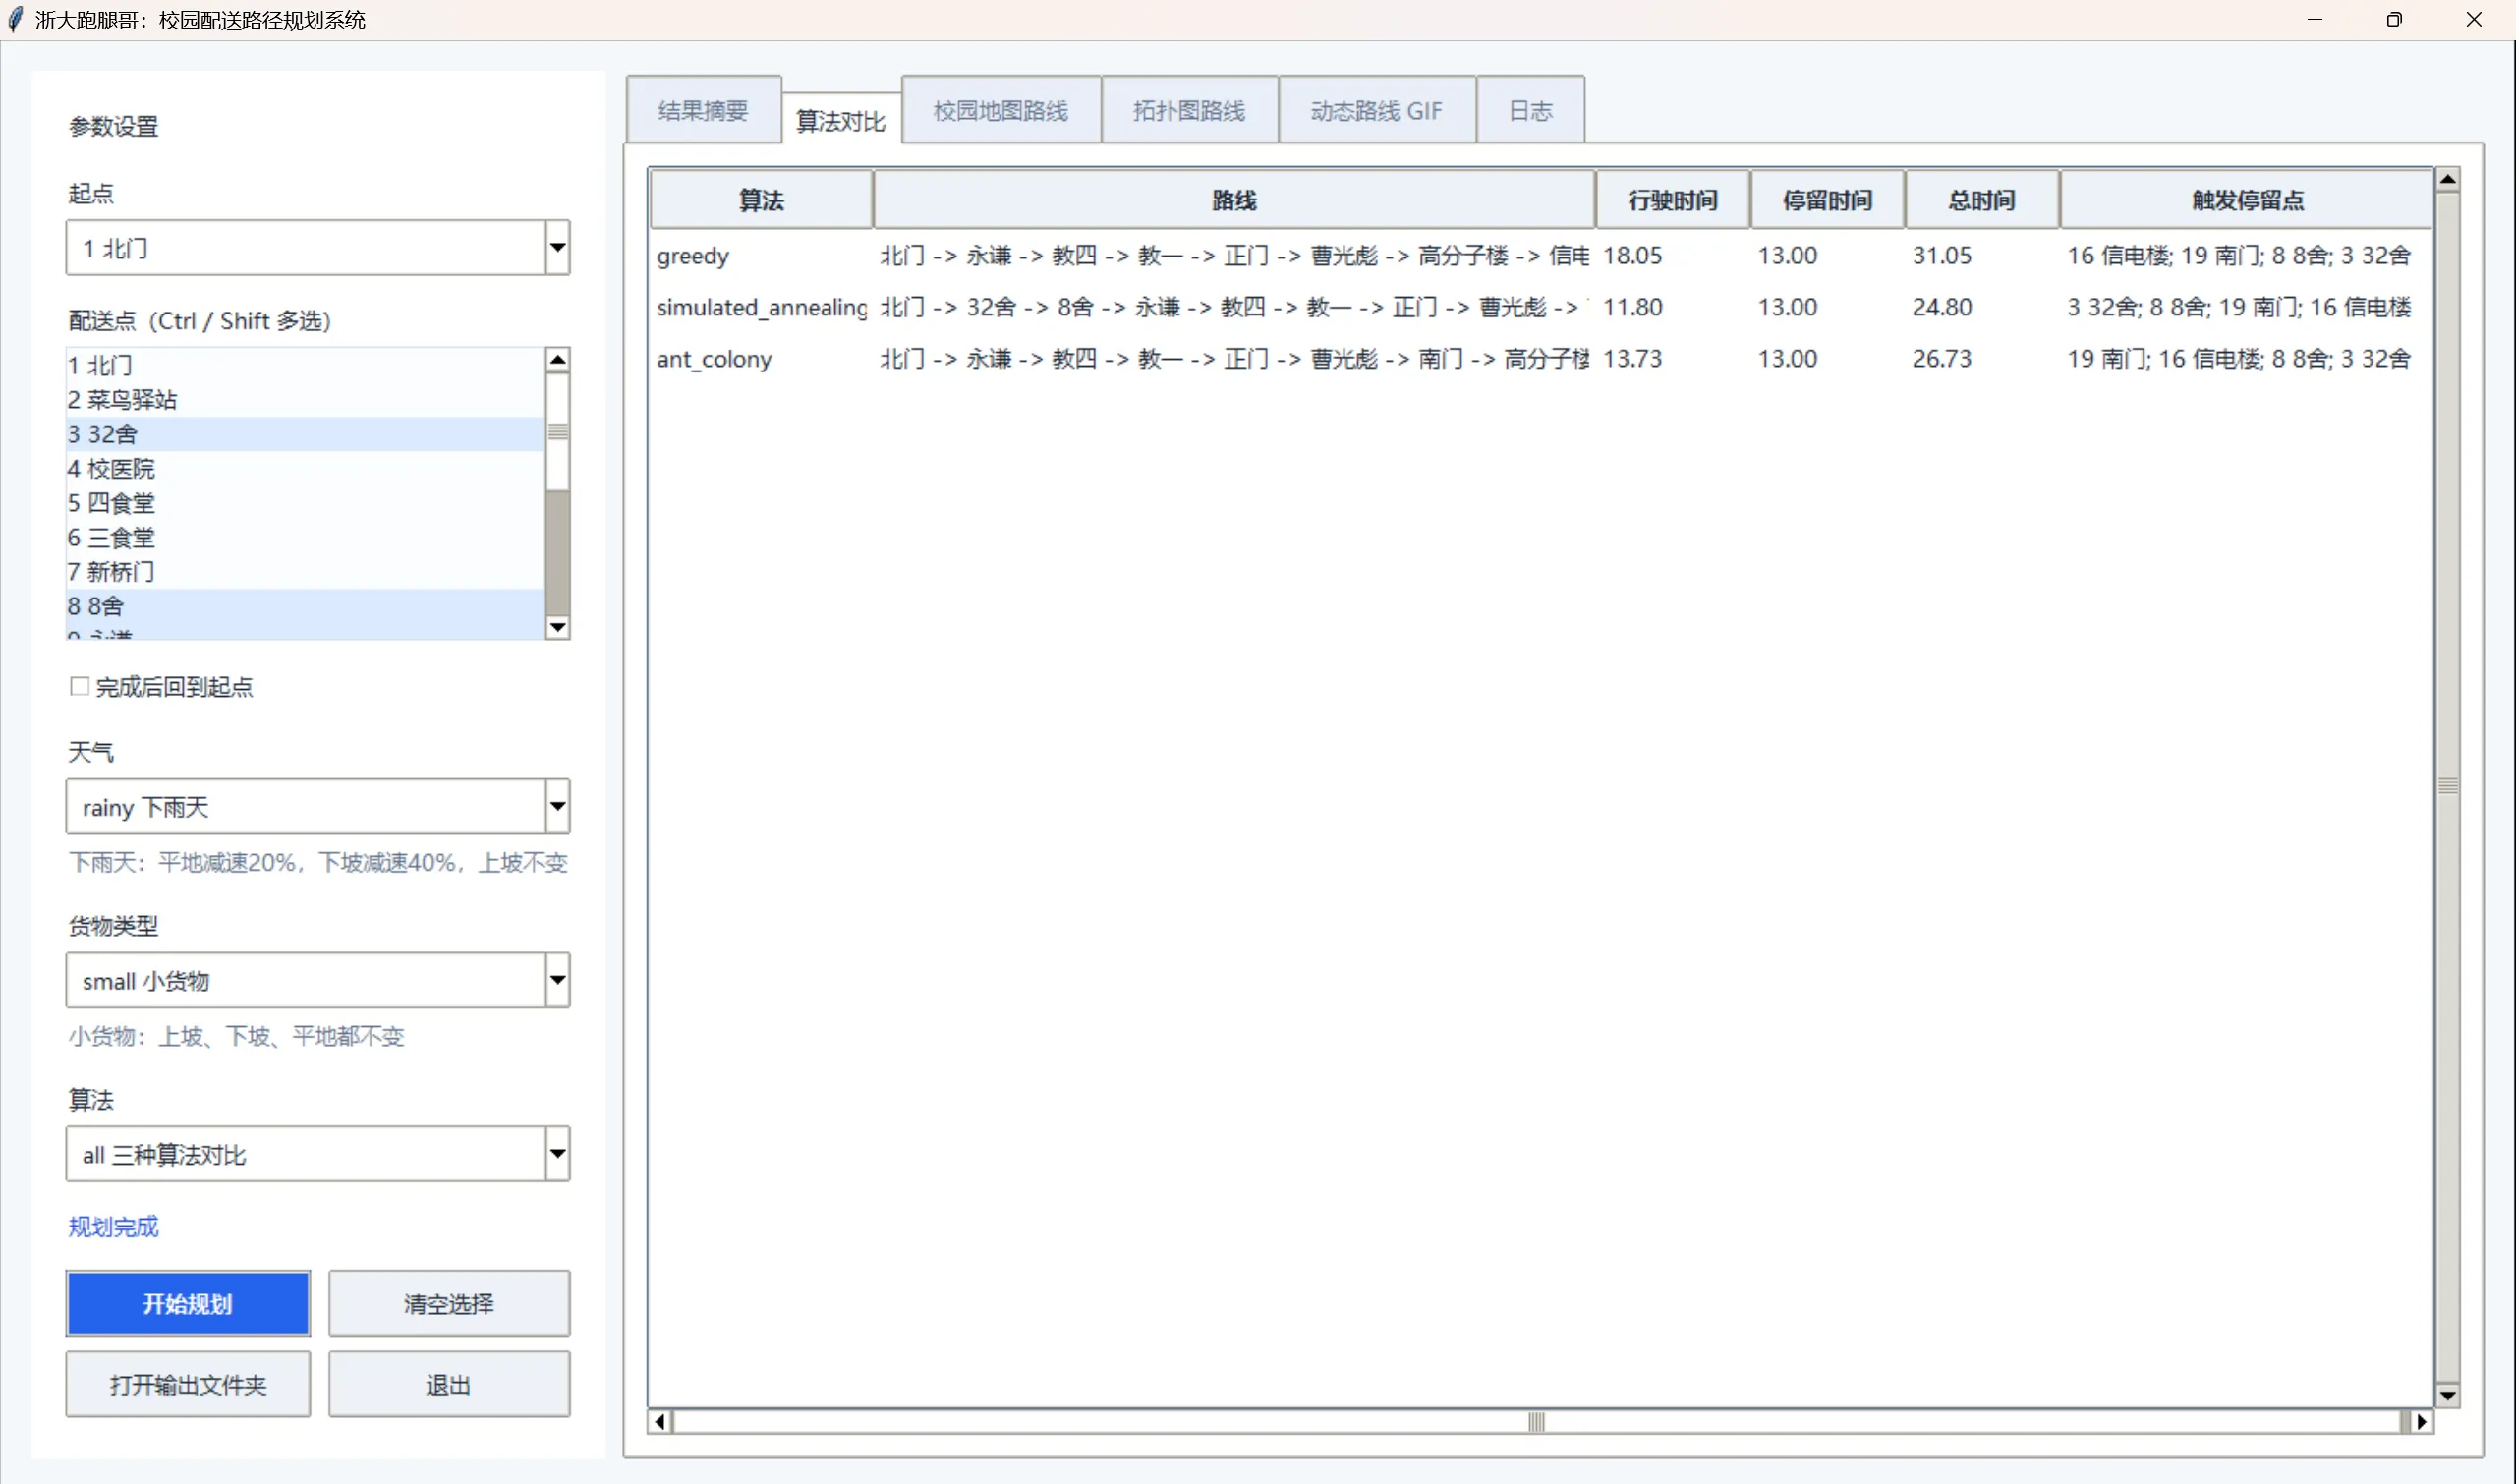
\includegraphics[width=0.98\textwidth]{figures/report_weather_complex_rainy_compare.png}
    \caption{下雨天情景下的三种算法对比结果}
    \label{fig:rainy_algo_compare}
\end{figure}

\begin{table}[H]
\centering
\caption{下雨天情景下三种算法数值对比}
\label{tab:rainy_algo_compare}
\small
\begin{tabularx}{\textwidth}{c|X|c|c|c}
\hline
算法 & 路线 & 行驶时间/min & 停留时间/min & 总时间/min \\
\hline
Greedy & 北门 $\rightarrow$ 永谦 $\rightarrow$ 教四 $\rightarrow$ 教一 $\rightarrow$ 正门 $\rightarrow$ 曹光彪 $\rightarrow$ 高分子楼 $\rightarrow$ 信电楼 & 18.05 & 13.00 & 31.05 \\
\hline
Simulated Annealing & 北门 $\rightarrow$ 32舍 $\rightarrow$ 8舍 $\rightarrow$ 永谦 $\rightarrow$ 教四 $\rightarrow$ 教一 $\rightarrow$ 正门 $\rightarrow$ 曹光彪 & 11.80 & 13.00 & 24.80 \\
\hline
Ant Colony & 北门 $\rightarrow$ 永谦 $\rightarrow$ 教四 $\rightarrow$ 教一 $\rightarrow$ 正门 $\rightarrow$ 曹光彪 $\rightarrow$ 南门 $\rightarrow$ 高分子楼 & 13.73 & 13.00 & 26.73 \\
\hline
\end{tabularx}
\end{table}

\begin{figure}[H]
    \centering
    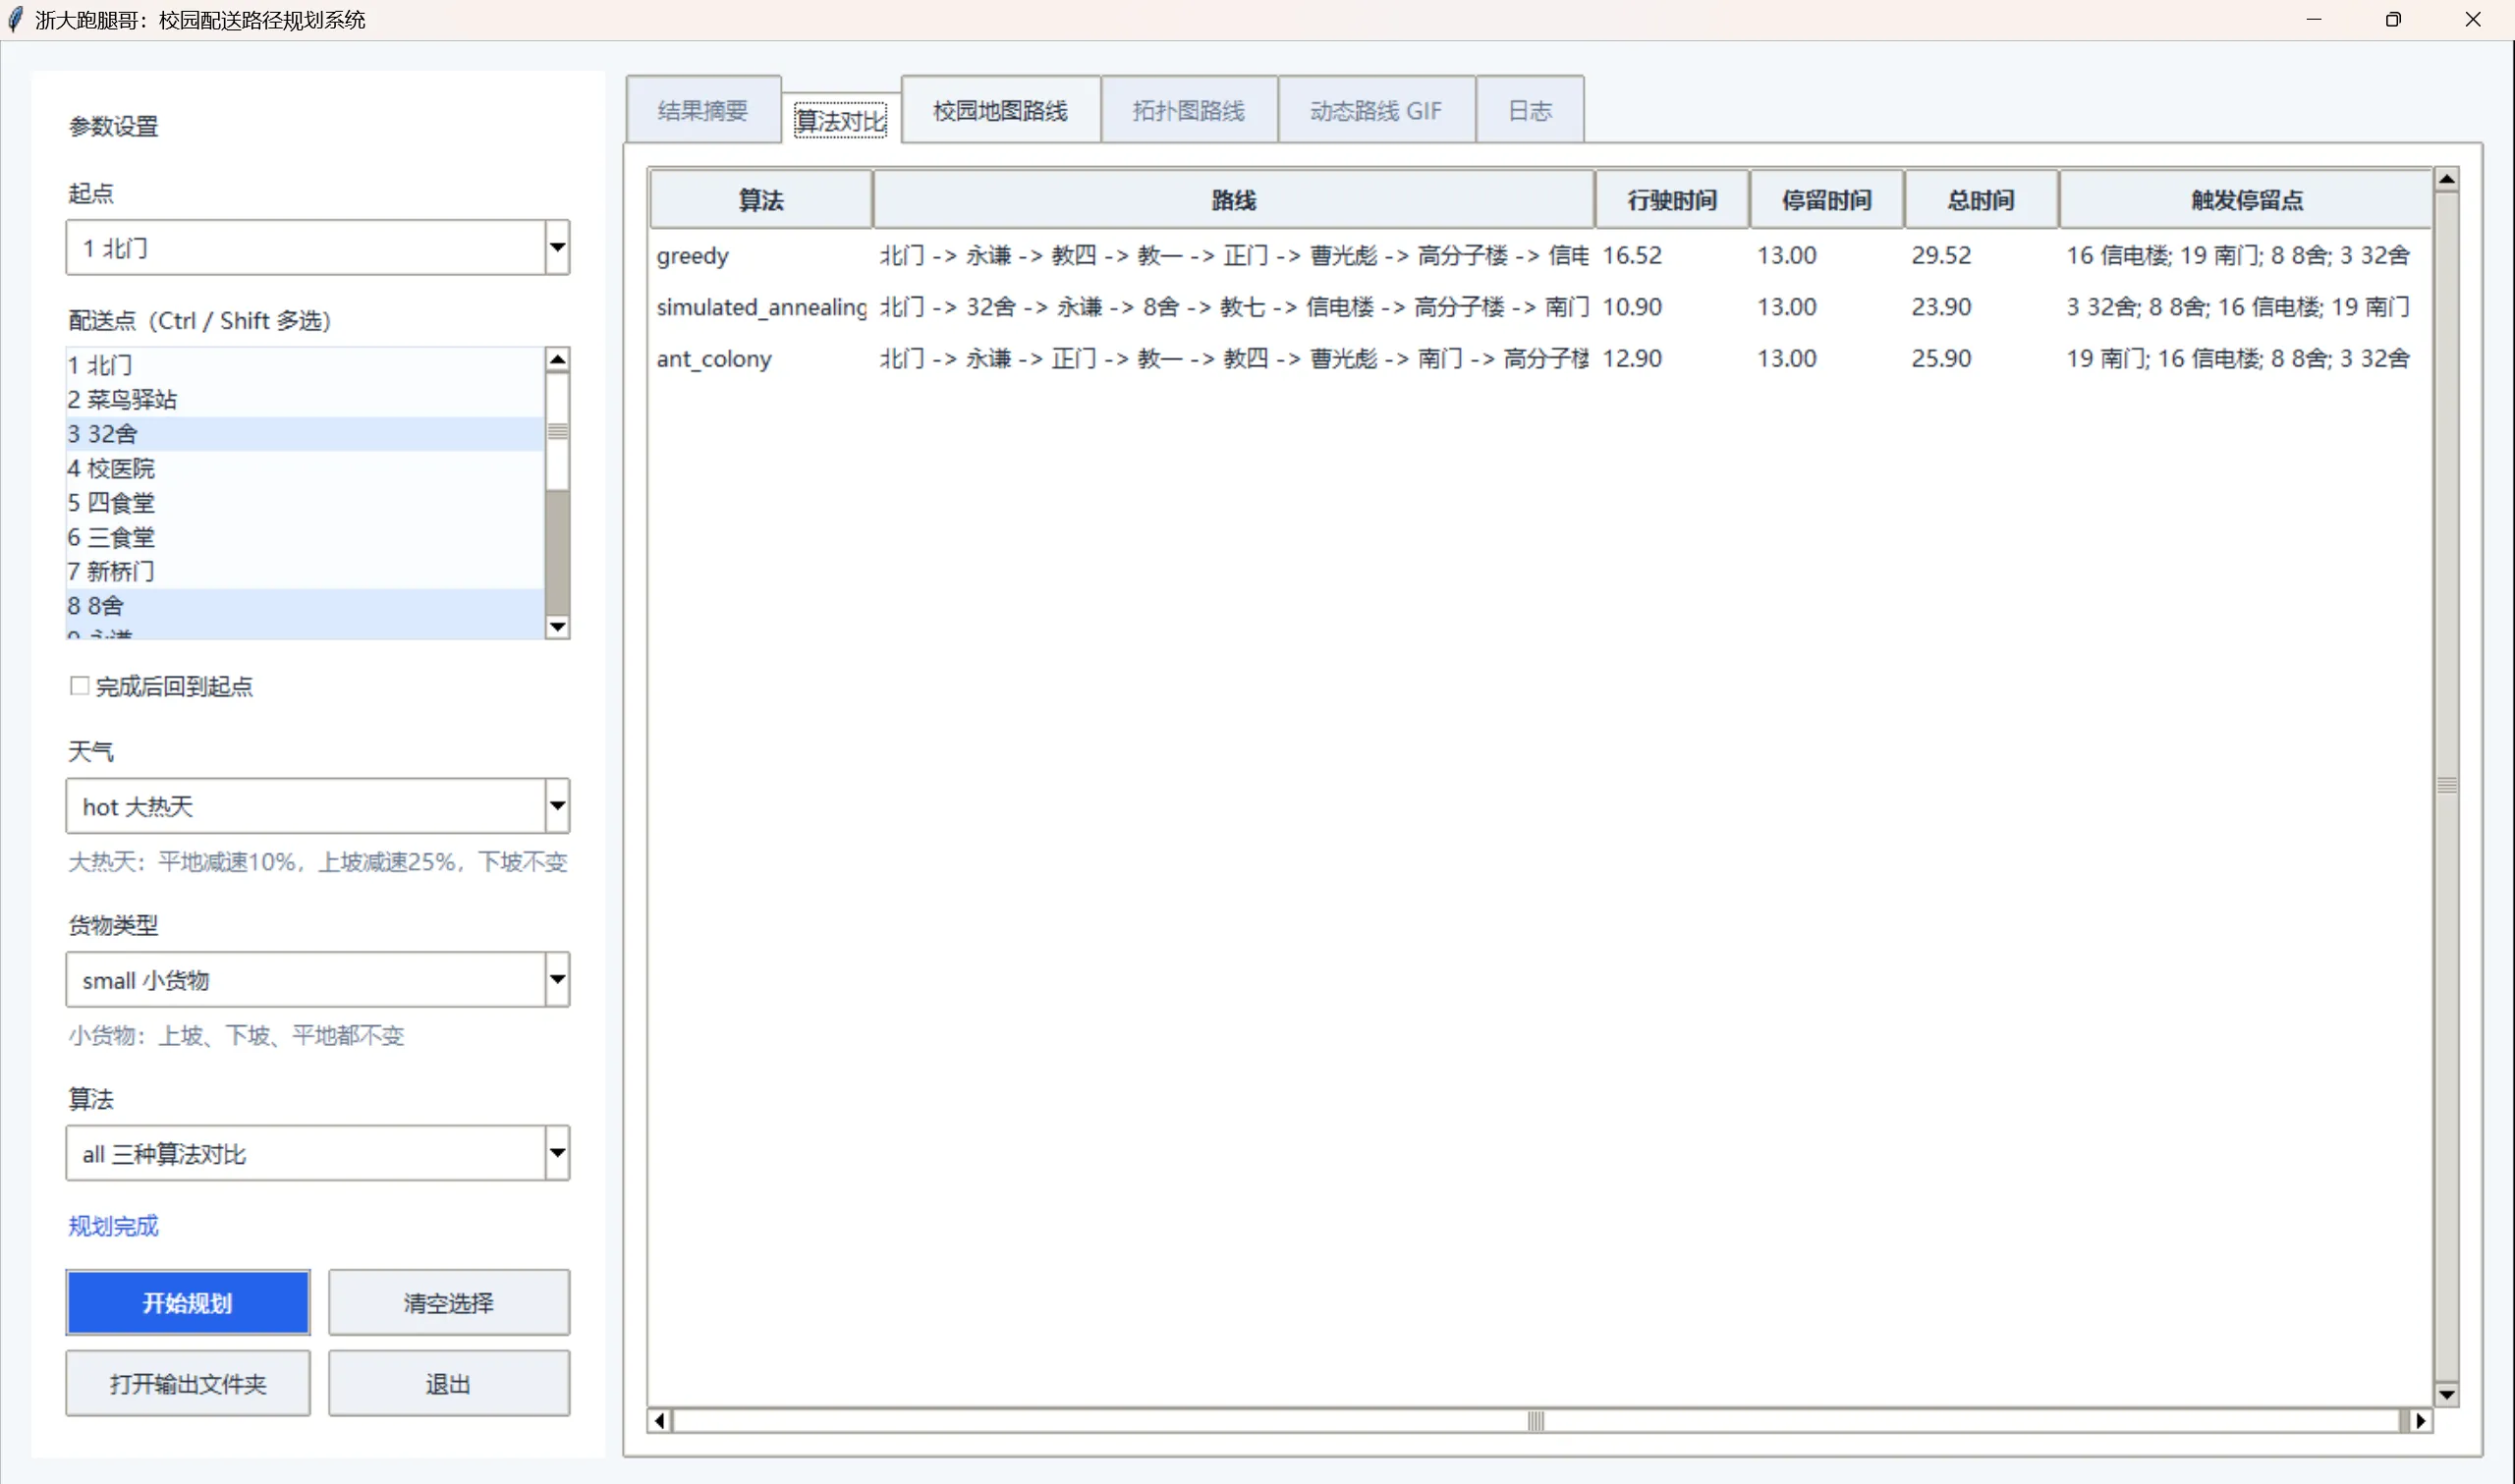
\includegraphics[width=0.98\textwidth]{figures/report_weather_complex_hot_compare.png}
    \caption{大热天情景下的三种算法对比结果}
    \label{fig:hot_algo_compare}
\end{figure}

\begin{table}[H]
\centering
\caption{大热天情景下三种算法数值对比}
\label{tab:hot_algo_compare}
\small
\begin{tabularx}{\textwidth}{c|X|c|c|c}
\hline
算法 & 路线 & 行驶时间/min & 停留时间/min & 总时间/min \\
\hline
Greedy & 北门 $\rightarrow$ 永谦 $\rightarrow$ 教四 $\rightarrow$ 教一 $\rightarrow$ 正门 $\rightarrow$ 曹光彪 $\rightarrow$ 高分子楼 $\rightarrow$ 信电楼 & 16.52 & 13.00 & 29.52 \\
\hline
Simulated Annealing & 北门 $\rightarrow$ 32舍 $\rightarrow$ 永谦 $\rightarrow$ 8舍 $\rightarrow$ 教七 $\rightarrow$ 信电楼 $\rightarrow$ 高分子楼 $\rightarrow$ 南门 & 10.90 & 13.00 & 23.90 \\
\hline
Ant Colony & 北门 $\rightarrow$ 永谦 $\rightarrow$ 正门 $\rightarrow$ 教一 $\rightarrow$ 教四 $\rightarrow$ 曹光彪 $\rightarrow$ 南门 $\rightarrow$ 高分子楼 & 12.90 & 13.00 & 25.90 \\
\hline
\end{tabularx}
\end{table}

从表 \ref{tab:rainy_algo_compare} 和表 \ref{tab:hot_algo_compare} 可以进一步看出，贪心算法虽然能够快速生成可行路线，但它每一步只依据当前局部增量进行选择，因此在复杂情景下可能产生较长路线。模拟退火和蚁群算法通过全局搜索或群体搜索机制，通常能够获得更低的总配送时间。


\subsection{三种算法与精确最优路径对比}

为了验证启发式算法在小规模任务中的解质量，本项目还使用状态压缩动态规划算法进行精确最优解对照。图 \ref{fig:x_algo_compare} 展示了 X 路径任务中三种启发式算法的对比结果，图 \ref{fig:x_exact_path} 展示了同一任务下精确 DP 得到的最优路径结果。

\begin{figure}[H]
    \centering
    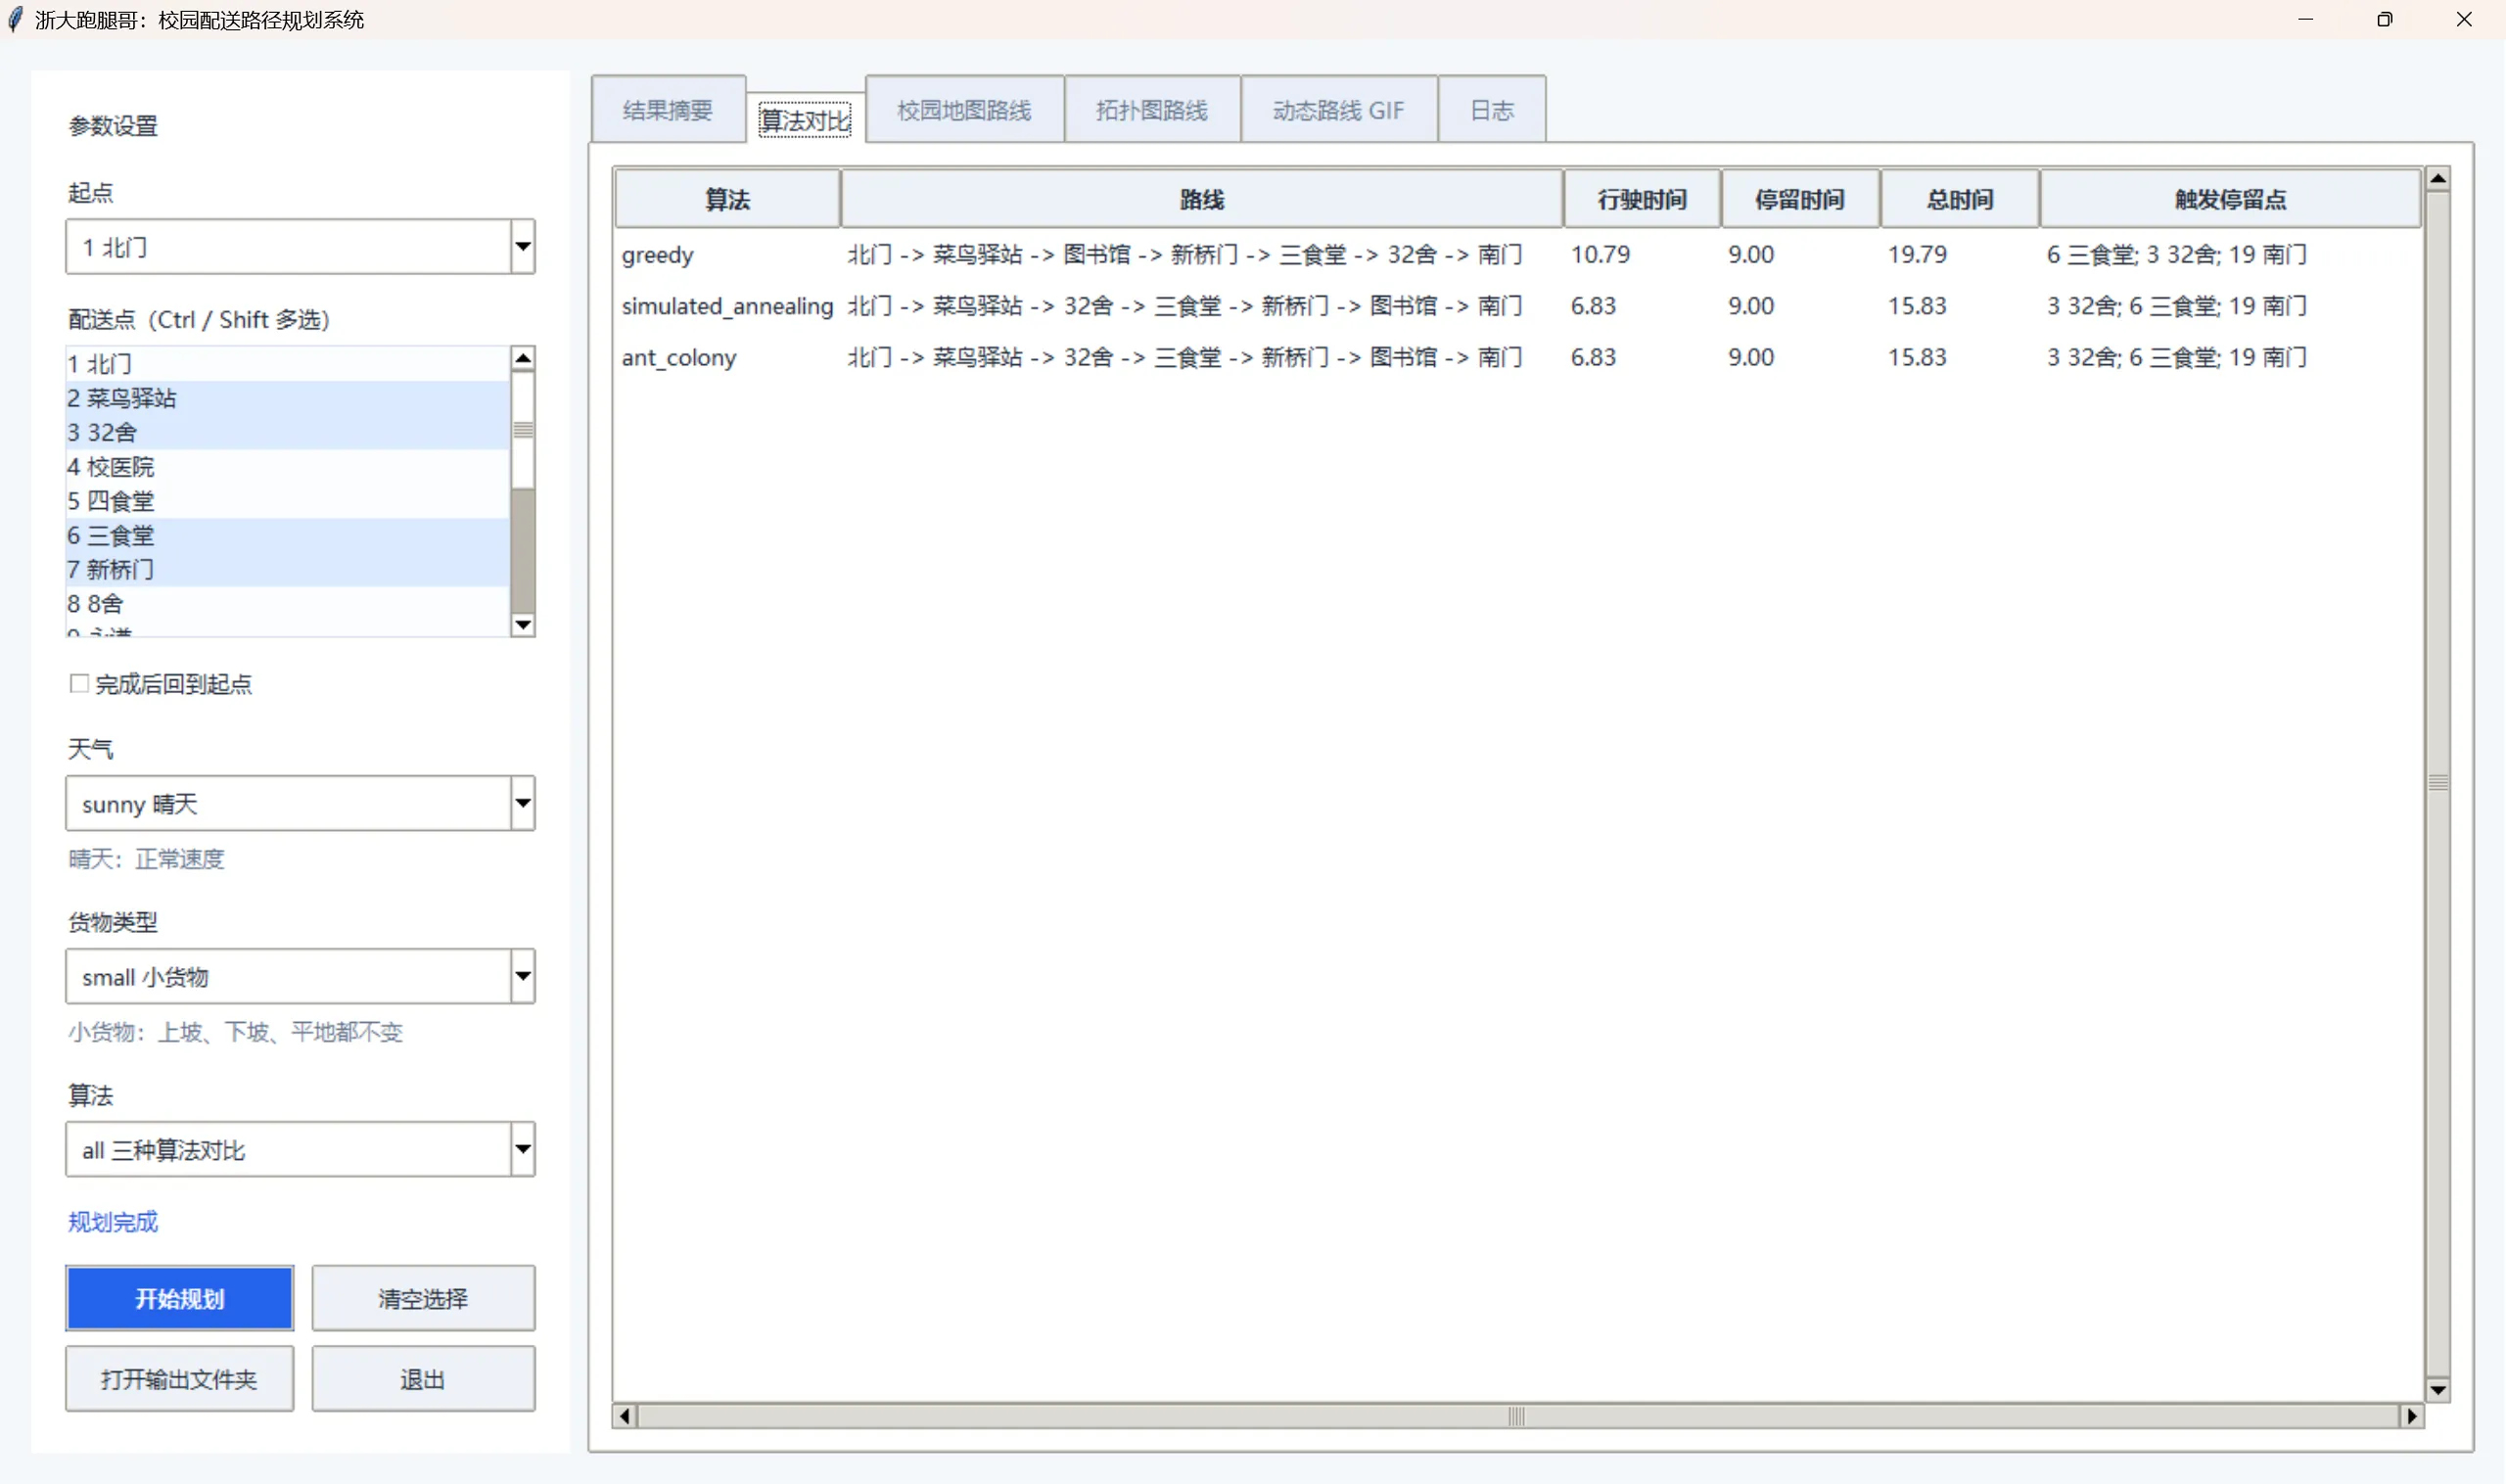
\includegraphics[width=0.98\textwidth]{figures/report_x_algo_compare.png}
    \caption{X 路径任务中的三种启发式算法对比结果}
    \label{fig:x_algo_compare}
\end{figure}

\begin{table}[H]
\centering
\caption{X 路径任务三种启发式算法数值对比}
\label{tab:x_algo_compare}
\small
\begin{tabularx}{\textwidth}{c|X|c|c|c}
\hline
算法 & 路线 & 行驶时间/min & 停留时间/min & 总时间/min \\
\hline
Greedy & 北门 $\rightarrow$ 菜鸟驿站 $\rightarrow$ 图书馆 $\rightarrow$ 新桥门 $\rightarrow$ 三食堂 $\rightarrow$ 32舍 $\rightarrow$ 南门 & 10.79 & 9.00 & 19.79 \\
\hline
Simulated Annealing & 北门 $\rightarrow$ 菜鸟驿站 $\rightarrow$ 32舍 $\rightarrow$ 三食堂 $\rightarrow$ 新桥门 $\rightarrow$ 图书馆 $\rightarrow$ 南门 & 6.83 & 9.00 & 15.83 \\
\hline
Ant Colony & 北门 $\rightarrow$ 菜鸟驿站 $\rightarrow$ 32舍 $\rightarrow$ 三食堂 $\rightarrow$ 新桥门 $\rightarrow$ 图书馆 $\rightarrow$ 南门 & 6.83 & 9.00 & 15.83 \\
\hline
\end{tabularx}
\end{table}

\begin{figure}[H]
    \centering
    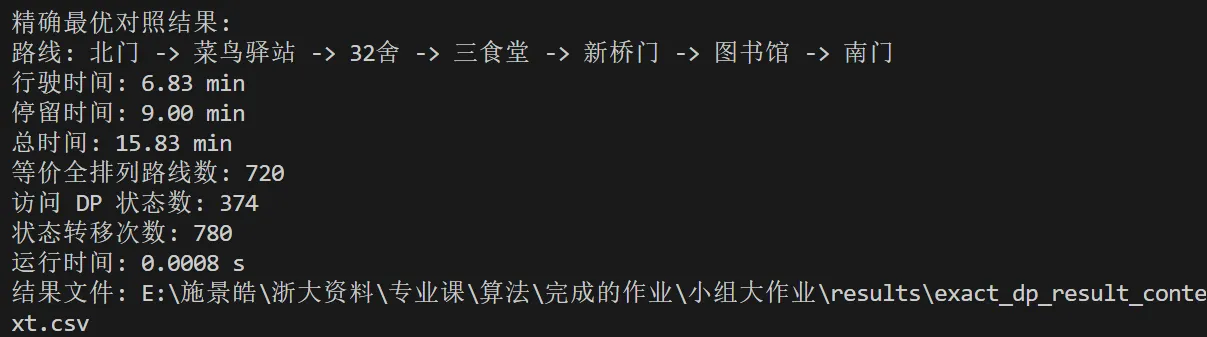
\includegraphics[width=0.98\textwidth]{figures/report_x_exact_path.png}
    \caption{X 路径任务中状态压缩 DP 得到的精确最优路径}
    \label{fig:x_exact_path}
\end{figure}

\begin{table}[H]
\centering
\caption{X 路径任务精确 DP 对照结果}
\label{tab:x_exact_dp}
\small
\begin{tabularx}{\textwidth}{c|>{\centering\arraybackslash}X}
\hline
项目 & 结果 \\
\hline
最优路线 & 北门 $\rightarrow$ 菜鸟驿站 $\rightarrow$ 32舍 $\rightarrow$ 三食堂 $\rightarrow$ 新桥门 $\rightarrow$ 图书馆 $\rightarrow$ 南门 \\
\hline
行驶时间 & 6.83 min \\
\hline
停留时间 & 9.00 min \\
\hline
总时间 & 15.83 min \\
\hline
等价全排列路线数 & 720 \\
\hline
访问 DP 状态数 & 374 \\
\hline
状态转移次数 & 780 \\
\hline
运行时间 & 0.001002 s \\
\hline
\end{tabularx}
\end{table}

由表 \ref{tab:x_algo_compare} 和表 \ref{tab:x_exact_dp} 可知，模拟退火算法和蚁群算法在该小规模测试任务中均找到了与精确 DP 一致的最优路线，总时间为 15.83 min，明显优于最近邻贪心算法的 19.79 min。这说明贪心算法虽然具有较高的运行效率，但在多配送点任务中容易受到局部选择的限制；相比之下，模拟退火和蚁群算法具有更强的全局搜索能力。

需要说明的是，此处“最优”指的是在当前建模假设下的最优，即基于本项目构造的道路拓扑、距离标注、坡度系数、天气与货物修正系数以及地点停留惩罚规则得到的最优解，并不等同于现实世界中考虑实时人流、车辆状态和道路管制后的绝对最优路线。




\section{复杂度分析}

本节从道路图规模和配送任务规模两方面分析项目中主要算法的复杂度。设道路节点数为 $n$，有向边数为 $m$，配送点数量为 $k$，两配送点之间最短路径平均展开长度为 $l$，模拟退火候选解评价次数为 $S$，蚁群算法蚂蚁数量为 $A$，蚁群迭代轮数为 $I$，特殊停留节点数量为 $h$。当前项目中 $n=59$，$m=162$。

项目的总代价函数为
\[
    total\_time = drive\_time + delay\_time
\]
其中，$drive\_time$ 由最短路矩阵查询得到，$delay\_time$ 由完整路径中触发的特殊地点停留惩罚组成。因此，复杂度分析需要同时考虑矩阵查询和路径展开。

\subsection{道路边权与路线评价}

情景边权更新需要遍历所有有向边，并根据坡度、天气和货物重量重新计算边代价，因此时间复杂度为 $O(m)$，空间复杂度为 $O(m)$。给定一条候选配送路线时，相邻配送点之间的行驶时间可以通过矩阵 $O(1)$ 查询，但还需要展开路径判断是否经过特殊停留节点。若平均展开长度为 $l$，配送点数量为 $k$，则单次路线评价复杂度为 $O(kl)$，用于记录已触发停留节点的空间复杂度约为 $O(h)$。

\subsection{Dijkstra 预处理}

单源 Dijkstra 使用邻接表和堆优化优先队列实现，时间复杂度为 $O((n+m)\log n)$，空间复杂度为 $O(n+m)$。由于项目需要任意两点之间的最短路，需要对每个节点运行一次 Dijkstra，因此全源预处理时间复杂度为
\[
    O(n(n+m)\log n)
\]
并额外保存代价矩阵和路径矩阵。其空间复杂度可写为
\[
    O(n+m+n^2+n^2l)
\]
这体现了用额外存储换取后续路线评价效率的思想。

\subsection{三种启发式算法}

最近邻贪心每一步都要在剩余配送点中寻找增量总代价最小的点。第 $r$ 轮需要比较 $r$ 个候选点，每个候选点需要展开路径计算新增停留惩罚，因此总体复杂度为
\[
    O(k^2l)
\]
空间复杂度为 $O(k+h)$。

模拟退火先用贪心生成初始路线，再通过 swap 和 reverse 产生候选路线。若共评价 $S$ 条候选路线，每条路线评价复杂度为 $O(kl)$，则主体复杂度为
\[
    O(Skl)
\]
若把贪心初始化也计入，则为 $O(k^2l)+O(Skl)$。空间上主要保存当前解、候选解和最优解，因此为 $O(k+h)$。

蚁群算法中，每只蚂蚁构造一条完整路线时，需要多次在剩余配送点中计算转移概率。单只蚂蚁的路线构造复杂度约为 $O(k^2l)$；若每轮有 $A$ 只蚂蚁，共迭代 $I$ 轮，则总时间复杂度为
\[
    O(IAk^2l)
\]
空间复杂度主要来自信息素矩阵和蚂蚁路径记录，约为 $O(k^2+Ak)$。

\subsection{状态压缩 DP}

若只考虑配送点访问集合和当前位置，状态压缩 DP 的典型复杂度为 $O(2^k k^2)$。但本项目还需要记录哪些特殊停留节点已经触发过惩罚，因此状态中额外包含 $delay\_mask$。设特殊停留节点数量为 $h$，则理论时间复杂度上界为
\[
    O(2^k2^hk^2)
\]
空间复杂度上界为
\[
    O(2^k2^hk)
\]
因此精确 DP 不适合作为大规模主算法，只用于小规模任务的最优性验证。

\subsection{复杂度对比总结}

综合以上分析，项目中各算法和模块的复杂度如表 \ref{tab:complexity_summary} 所示。

\begin{table}[H]
\centering
\caption{主要算法和模块复杂度对比}
\label{tab:complexity_summary}
\small
\renewcommand{\arraystretch}{1.2}
\begin{tabularx}{\textwidth}{c|c|c|X}
\hline
模块或算法 & 时间复杂度 & 空间复杂度 & 说明 \\
\hline
情景边权更新 & $O(m)$ & $O(m)$ & 遍历所有有向边，重新计算天气和货物影响后的边权 \\
\hline
单源 Dijkstra & $O((n+m)\log n)$ & $O(n+m)$ & 从一个源点出发求到其他节点的最短路 \\
\hline
全源 Dijkstra 预处理 & $O(n(n+m)\log n)$ & $O(n+m+n^2+n^2l)$ & 对每个节点运行一次 Dijkstra，保存代价矩阵和路径矩阵 \\
\hline
单次路线评价 & $O(kl)$ & $O(h)$ & 查询最短路矩阵，并展开路径计算停留惩罚 \\
\hline
最近邻贪心 & $O(k^2l)$ & $O(k+h)$ & 每一步选择当前增量总代价最小的配送点 \\
\hline
模拟退火 & $O(k^2l)+O(Skl)$ & $O(k+h)$ & 贪心初始化后进行 $S$ 次邻域搜索 \\
\hline
蚁群算法 & $O(IAk^2l)$ & $O(k^2+Ak)$ & 每轮 $A$ 只蚂蚁构造路线并更新信息素 \\
\hline
状态压缩 DP & $O(2^k2^hk^2)$ & $O(2^k2^hk)$ & 同时记录访问配送点集合和已触发停留节点集合 \\
\hline
\end{tabularx}
\end{table}

从表 \ref{tab:complexity_summary} 可以看出，道路层 Dijkstra 预处理主要受 $n$ 和 $m$ 影响，而配送顺序优化主要受 $k$ 和 $l$ 影响。贪心算法复杂度较低，但容易陷入局部最优；模拟退火和蚁群算法增加了迭代搜索的开销，但能得到更好的路线质量；精确 DP 可以给出小规模任务的最优解，但由于 $2^k$ 和 $2^h$ 的存在，随着配送点数量和特殊停留节点数量增加，复杂度会迅速上升。

因此，本项目最终采用：
\[
    \text{道路层 Dijkstra 预处理}
    +
    \text{配送层启发式优化}
    +
    \text{小规模 DP 精确验证}
\]
的整体结构。这样既可以利用预处理矩阵降低路线评价成本，又可以利用模拟退火和蚁群算法在可接受时间内搜索较优路线，同时还能用 DP 对小规模任务进行精确验证。




\section{可视化与交互界面}

项目最终实现了基于 Tkinter 的交互界面。用户可以在界面中选择起点、配送点、天气、货物重量和算法类型，系统自动生成情景代价矩阵、运行算法并输出结果。界面包含结果摘要、算法对比、校园地图路线、拓扑图路线、动态路线 GIF 和运行日志等标签页。

\begin{figure}[H]
    \centering
    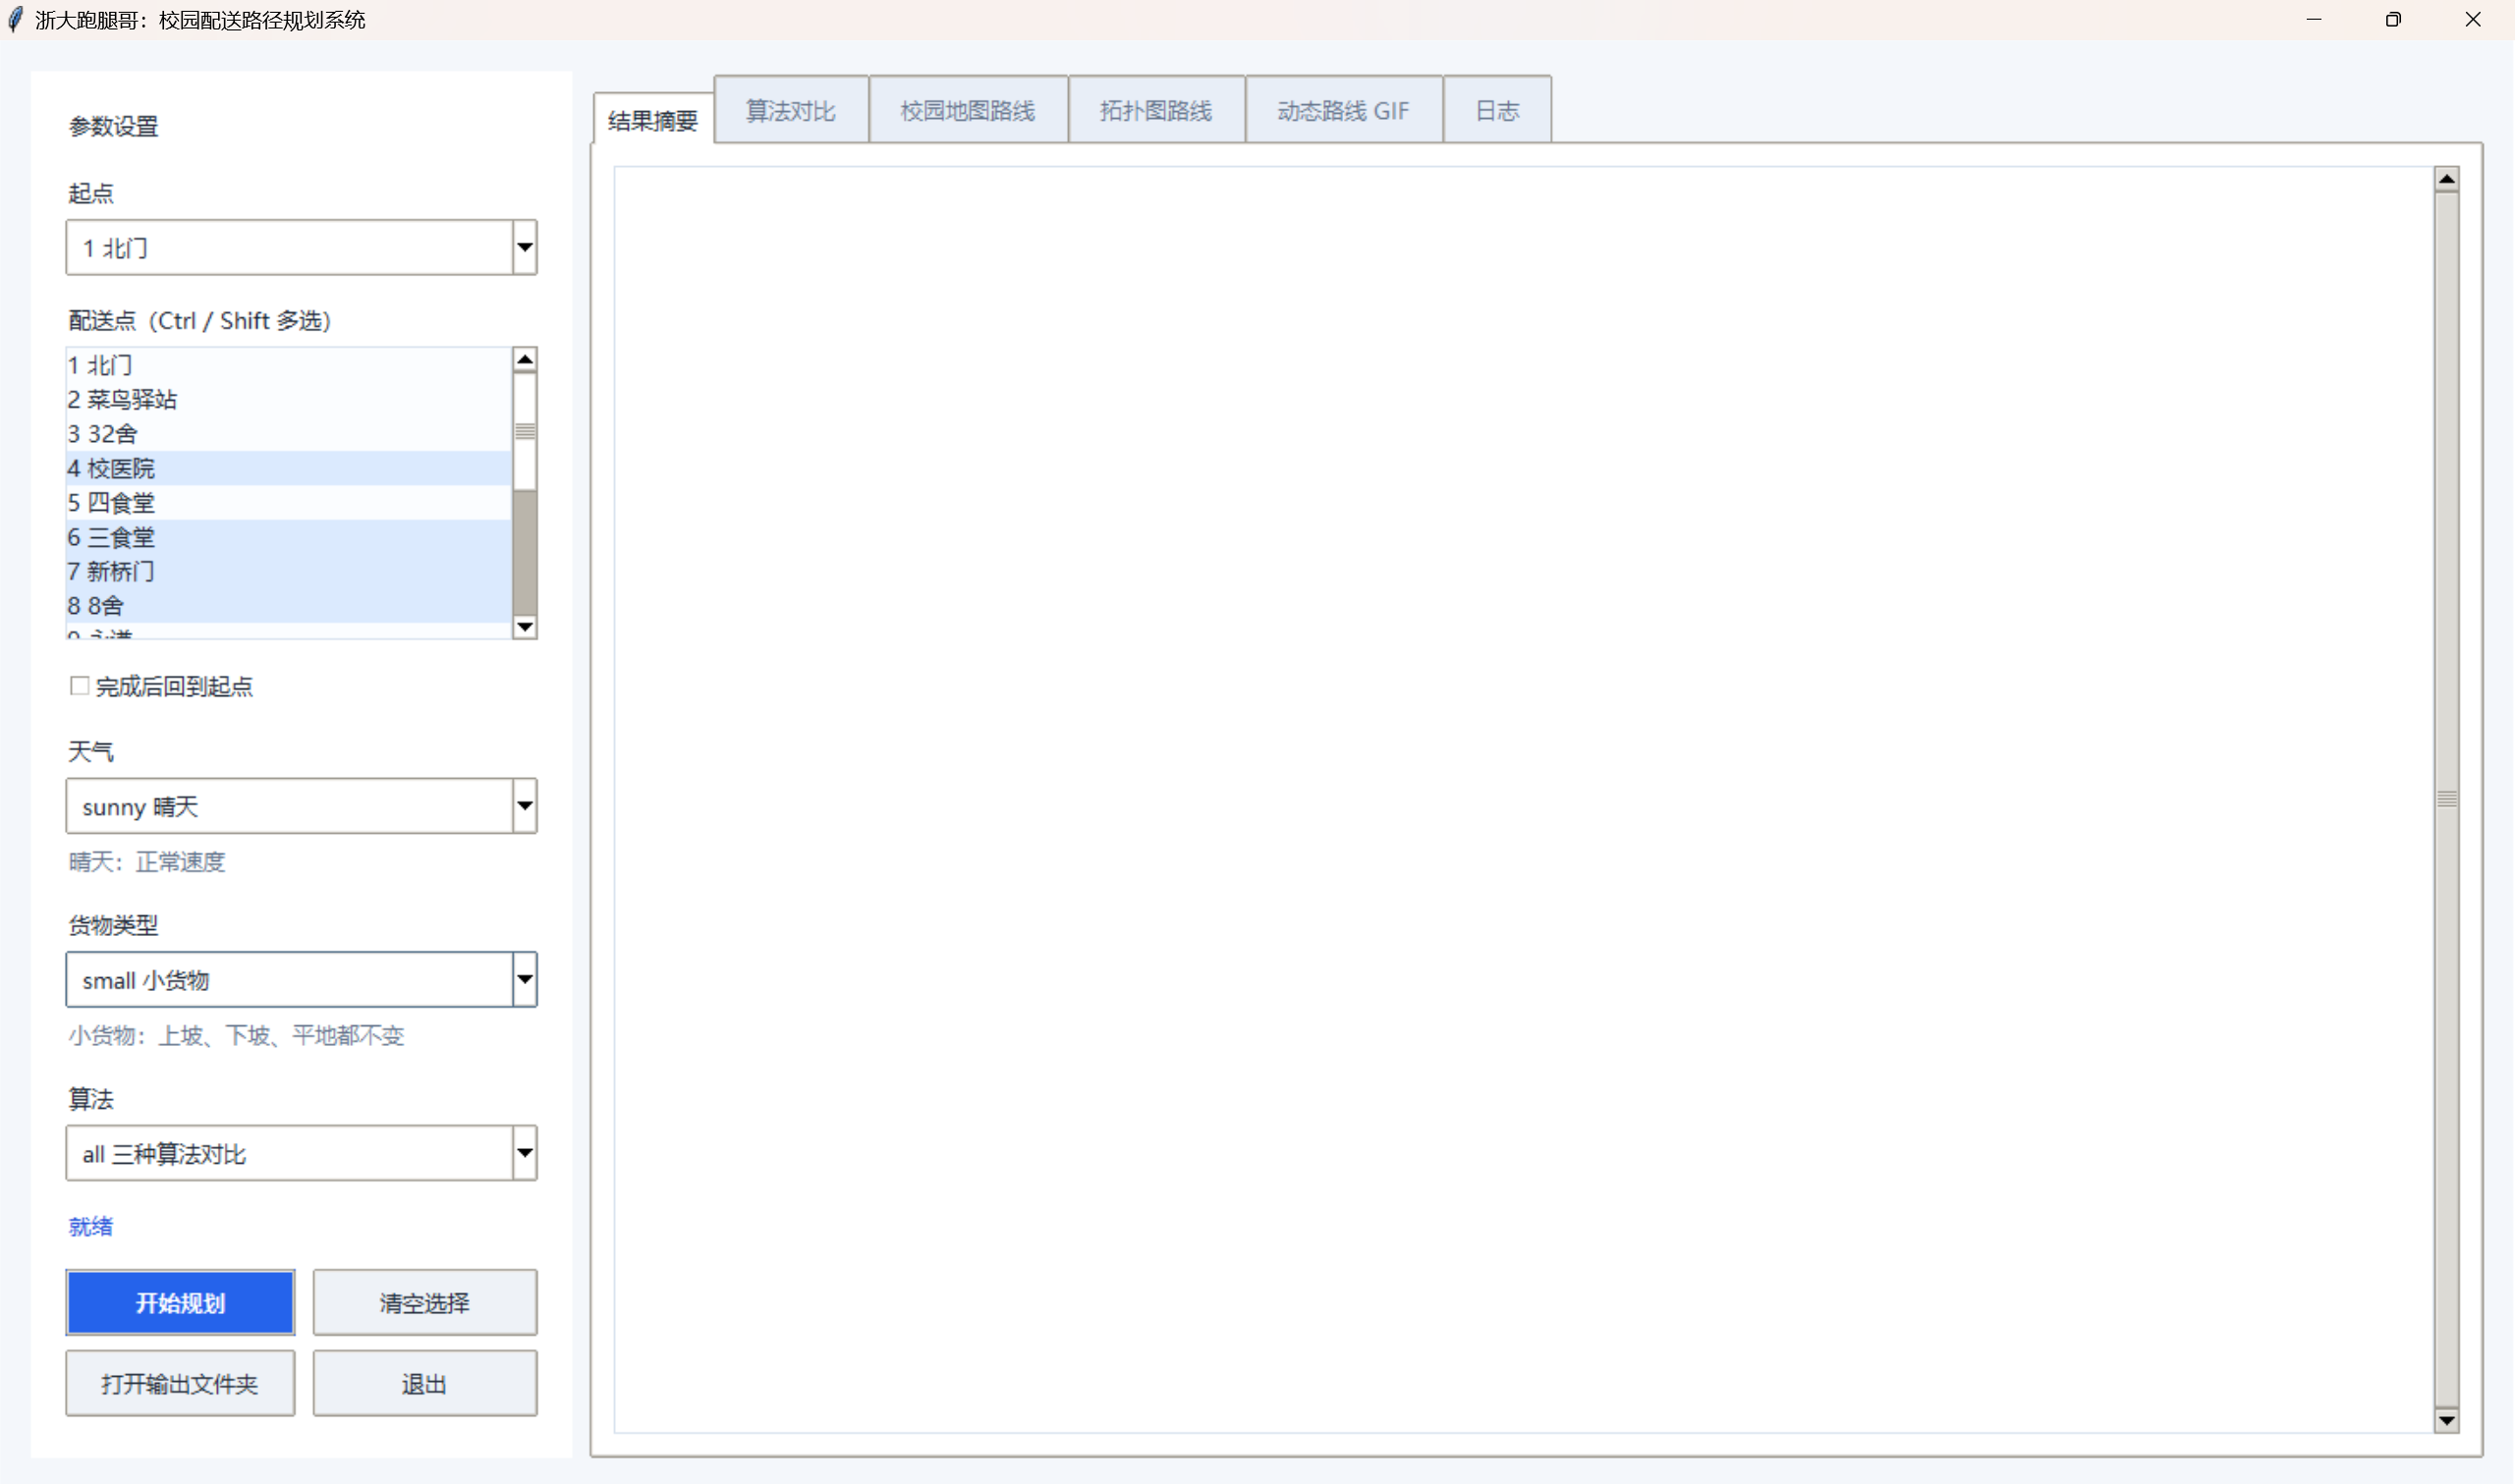
\includegraphics[width=0.85\textwidth]{figures/report_ui_overall.png}
    \caption{校园配送路径规划系统整体交互界面}
    \label{fig:ui_overall}
\end{figure}

路线可视化模块会读取 \texttt{edges\_raw.csv} 中记录的像素线段，将算法得到的配送访问顺序通过 \texttt{context\_path\_matrix.json} 展开为完整经过节点序列，再绘制到校园地图和拓扑图上。由于 LaTeX 通常不能直接插入 GIF 动画，报告中插入静态路线图，动态文件 \texttt{route/route\_animation.gif} 可作为课堂展示材料。

系统输出的三类可视化结果含义不同，如表 \ref{tab:visual_outputs} 所示。卫星地图路线用于展示路线在真实校园中的空间位置，拓扑图路线用于展示算法实际使用的抽象道路结构，动态 GIF 则用于课堂展示路线行进过程。

\begin{table}[H]
\centering
\caption{路线可视化输出说明}
\label{tab:visual_outputs}
\small
\renewcommand{\arraystretch}{1.2}
\begin{tabularx}{0.92\textwidth}{c|X}
\hline
输出文件 & 作用 \\
\hline
\texttt{route/route\_on\_yuquan\_map.png} & 在校园卫星地图上展示最终推荐路线的位置与走向 \\
\hline
\texttt{route/route\_on\_topology\_slope\_check.png} & 在抽象拓扑图上展示算法实际使用的道路节点和连接关系 \\
\hline
\texttt{route/route\_animation.gif} & 以动画方式展示路线行进过程，适合课堂演示 \\
\hline
\end{tabularx}
\end{table}

\section{分工说明}

本项目为三人小组合作完成。根据课堂展示材料和项目实际工作内容，小组成员分工如表所示。

\begin{table}[H]
\centering
\caption{小组成员分工}
\begin{tabularx}{\textwidth}{c|X|c}
\hline
成员 & 主要工作 & 贡献比例 \\
\hline
施景皓 & 负责算法设计与主要代码实现，包括图建模流程、Dijkstra 预处理、路径优化算法、精确 DP 验证和 UI/可视化整合。 & 1/3 \\
\hline
吴溪语 & 负责代码调试、实验结果核对与报告撰写，参与数据整理和结果分析。 & 1/3 \\
\hline
孙钰淳 & 负责代码调试、PPT 制作与课堂展示材料整理，参与可视化结果和实验材料汇总。 & 1/3 \\
\hline
\end{tabularx}
\end{table}

三位成员贡献比例基本一致，分别承担算法实现、调试验证、报告与展示材料整理等任务。

\section{总结与不足}

本项目完成了从玉泉校区地图到校园配送路径规划系统的完整流程。首先，项目将地图抽象为包含 59 个节点、162 条有向边的加权图；其次，通过手写 Dijkstra 算法生成基础和情景最短路矩阵；然后，在配送顺序层面实现贪心、模拟退火和蚁群算法，并用状态压缩 DP 对小规模任务进行精确最优解验证；最后，实现了交互式 UI 和路线可视化功能。

从实验结果看，贪心算法具有较快的响应速度，但容易受局部选择限制；模拟退火和蚁群算法能够在当前测试任务中找到与精确 DP 一致的最优路线，说明启发式优化方法在该问题上具有较好的效果。项目没有使用 \texttt{networkx} 等现成图算法库完成核心算法，Dijkstra、贪心、模拟退火、蚁群算法和精确 DP 均为项目内实现。

项目仍存在一些不足。第一，道路拓扑来自人工标注，若道路边缺失或距离标注有误，算法结果会受到影响；第二，天气、货物和停留惩罚参数是规则化设定，并非来自真实统计数据；第三，当前精确 DP 只适合小规模任务；第四，系统尚未考虑实时交通、红绿灯、拥堵和不同交通工具速度差异。后续可以通过采集更多真实配送数据、优化参数设定和扩展多目标优化模型进一步改进。



\end{document}
